\documentclass[12pt]{article}
\usepackage[utf8x]{inputenc}
\usepackage{amsmath}
\usepackage{amsfonts}
\usepackage{mathrsfs}
\usepackage{natbib}
\usepackage{graphicx} % figuras
\usepackage[export]{adjustbox} % loads also graphicx
\usepackage{float}
\usepackage[font=footnotesize]{caption}
\usepackage{wrapfig}
\usepackage{authblk}
\usepackage{subfigure}
\usepackage{pifont}
\usepackage{a4wide}

\numberwithin{equation}{section}
%\usepackage{lipsum}
\topmargin=-2pt
\title{Name?}

\author[1]{G. B. Diaz Cortes}  
\author[1]{C. Vuik} 
\author[2]{J. D. Jansen} 
\affil[1]{Department of Applied Mathematics, TU Delft}
\affil[2]{Department of Geoscience \& Engineering, TU Delft}
\renewcommand\Authands{ and }
\date{March 2016}
\begin{document}



% Title Page

\maketitle
\begin{abstract}
     We study fast and robust iterative solvers for large systems of  linear equations resulting from reservoir simulation trough porous media. We propose the use of preconditioning and deflation techniques based on information obtained from the system to reduce the time spent in the solution of the linear system.\\
     An important question is to find good deflation vectors, which lead to a decrease in the number of iterations and a small increase in the required computing time per iteration. In this paper, the deflation vectors are based on a POD reduced set of snapshots. We investigate convergence and the properties of the resulting methods. Finally, we illustrate these theoretical results with numerical experiments.  
 We consider compressible and incompressible single-phase flow in a layered model with large variations in the permeability coefficients and the SPE10 benchmark model.\\
\end{abstract}

  \section{Introduction.}
  \hspace{0.5cm}Often, most computational time in the simulation of multi-phase flow through porous media is taken up by a
solution of the pressure equation. This involves primarily solving large systems of linear equations as 
part of the iterative solution of the time and space discretized governing nonlinear partial differential 
equations. The time spent in solving the linear systems depends on the size of the problem and the 
variations of permeability within the medium. Solution of problems with extreme contrasts in the grid block 
permeability values may lead to very large computing times.\\
A potential approach to reduce the computing time for large-scale problems with the aid of Proper Orthogonal 
Decomposition (POD) is investigated in \cite{Astrid11}, \cite{Mark06}, \cite{Pasetto16} and \cite{Carlberg15}. The use of a POD-based preconditioner for the acceleration of the solution is proposed by Astrid et al. \cite{Astrid11} to solve the pressure equation resulting from two-phase reservoir simulation, and by Pasetto et al. \cite{Pasetto16} for groundwater flow models. 
The POD method requires the computation of a series of 'snapshots' which are solutions of the problem with slightly different parameters or well inputs. Astrid et al. \cite{Astrid11} use as snapshots solutions of the pressure equation computed in a short number of pre-simulations previous to the actual simulation. Pasetto et al. \cite{Pasetto16} use as snapshots solutions of the previous time steps.
Once the snapshots are computed, the POD method is used to obtain a set of basis 
vectors that capture the most relevant features of the system, which can be used to speed-up the subsequent simulations.\\
A similar approach is used in \cite{Mark06}, where a set of POD-based 
basis vectors is obtained from the initial time steps. However, in this case, the acceleration is 
achieved by only improving the initial guess.\\
Problems with a high contrast between the permeability coefficients are sometimes approached through the 
use of deflation techniques; see, e.g., \cite{Vuik99}. The use of deflation techniques involves the search 
of good deflation vectors, which are usually problem-dependent. In \cite{Vuik99}, subdomain based deflation 
vectors are used for layered problems with a large contrast between the permeability coefficients. However, 
these deflation vectors cannot be used if the distribution of the permeability coefficients  is not 
structured as is the case in, e.g., the well-known SPE 10 benchmark problem \cite{Christie01}.\\
Following the ideas of \cite{Astrid11,Mark06,Pasetto16,Carlberg15}, we propose the use of POD of many snapshots to capture the system's behavior and combine this technique with deflation, to  accelerate the convergence of an iterative Krylov method. In \cite{Astrid11,Mark06} and \cite{Pasetto16}, after computing a basis from the previously obtained snapshots, the solution is computed in the subspace generated by this basis and then projected back to the original high dimensional system. In \cite{Carlberg15} POD is used to obtain information from the system, in particular, the previous time step solutions, and construct a Krylov-subspace containing the previously obtained information.
In this work, instead of computing the solution in the low dimension subspace, the basis obtained with POD is studied as an alternative choice of deflation vectors 
to accelerate the convergence of the pressure solution in reservoir simulation.  \\
  Section \ref{fpm} is devoted to a detailed description of the models used to simulate flow through a porous medium. In Section \ref{syseq} we give some theory about the linear solver used in this work and we introduce preconditioning and deflation techniques. We also prove two lemmas that will help us in the choice of good deflation vectors for the incompressible case, necessary for the deflation techniques.\\
 In Section \ref{numexp} we present numerical experiments. We describe the problem that is studied, the solver that is used and the preconditioning and deflation techniques used for the speedup of the solver. The results are also presented in this section. \\
 Finally, we end with the conclusions.
 
 
 \newpage
 \section{Flow through porous media}\label{fpm}
\hspace{0.5cm}Reservoir simulation is a way to analyze and predict the fluid behavior in a real reservoir
by the analysis of its behavior in a model. The description of subsurface flow simulation involves two types of models, mathematical and geological models. The geological model is used to describe the reservoir, i.e., the porous rock formation. 
The mathematical modeling of porous media flow is performed taking into account mass conservation, and Darcy's law
corresponding to the momentum conservation. The equations used to describe single-phase flow through a porous medium are:\\

\begin{equation}\label{eq:ce}
\frac{\partial (\rho \phi)}{\partial t}+ \nabla \cdot ( \rho \mathbf{v})=q, \qquad \mathbf{v}=-\frac{\mathbf{K}}{\mu}(\nabla \mathbf{p}-\rho g\nabla z),
\end{equation}
or
\begin{equation}\label{eq:ce1}
\frac{\partial (\rho \phi)}{\partial t}- \nabla \cdot \left( \frac{\rho\mathbf{K}}{\mu}(\nabla \mathbf{p}-\rho g\nabla z)\right)=q.
\end{equation}
Where the primary unknown is the pressure $\mathbf{p}$.  The fluid  $\rho=\rho(\mathbf{p})$ and rock $\phi=\phi(\mathbf{p})$ compressibilities can be pressure dependent.
Rock compressibility is defined by:
\begin{equation*}
 c_r=\frac{1}{\phi}\frac{d\phi}{dp}=\frac{ln(\phi)}{dp},
\end{equation*}
If the rock compressibility is constant, the previous equation can be integrated as:
\begin{equation*}
 \phi(p)=\phi_0 e^{c_r(p-p_0)}.
\end{equation*}
Fluid compressibility is defined as:
\begin{equation}\label{eq:fc}
 c_f=\frac{1}{\rho}\frac{d\rho}{dp}=\frac{ln(\rho)}{dp}.
\end{equation}
If the fluid compressibility is constant, the previous equation can be integrated as:
\begin{equation}\label{eq:rhoeq}
 \rho(\mathbf{p})=\rho_0 e^{c_f(\mathbf{p}-\mathbf{p}_0)}.
\end{equation}
Using implicit discretization, Equation \eqref{eq:ce} becomes:
\begin{equation}\label{eq:ce2}
 \frac{(\mathbf{\phi}\mathbf{\rho})^{n+1}-(\mathbf{\phi}\mathbf{\rho})^{n}}{\Delta t^n}
 +\nabla \cdot (\mathbf{\rho}(\mathbf{p}) \mathbf{v})^{n+1}=\mathbf{q}^{n},
\qquad
\mathbf{v}^{n+1}= -\frac{\mathbf{K}}{\mu^{n+1}}[\nabla(\mathbf{p}^{n+1})-g\mathbf{\rho}^{n+1}\nabla(\mathbf{z})],
\end{equation}
where $\mathbf{\rho}(\mathbf{p})$ is given by \ref{eq:rhoeq}.
If $\mathbf{\phi}$ and $\mathbf{\rho}$ depend nonlinearly on $\mathbf{p}$ we have a nonlinear system 
of equations to be solved for each time step.  \\
If in Equation \eqref{eq:ce2} the density and the porosity do not depend on the pressure and assuming no gravity terms, we have an incompressible model and we obtain a linear system given by:
\begin{equation}\label{eq:cel}
\nabla \cdot \left( -\mathbf{\rho}\frac{\mathbf{K}}{\mu}\nabla\mathbf{p}\right)=\mathbf{q},
\end{equation}
that after discretization can be written as:
 \begin{equation}\label{eq:cel1}
\mathbf{T}\mathbf{p} = \mathbf{q}.
\end{equation}
Where $\mathbf{T}$ is the transmissibility matrix.\\
If the density depends on the pressure assuming again no gravity terms, we have a compressible time-dependent problem and Equation \eqref{eq:ce2}
can be rewritten as:
\begin{equation}\label{eq:ce3}
 \frac{\mathbf{\phi}\mathbf{\rho}(\mathbf{p}^{n+1})
 -\mathbf{\phi}\mathbf{\rho}(\mathbf{p}^{n})}{\Delta t^n}
 +\nabla \cdot (\mathbf{\rho} \mathbf{v})^{n+1}=\mathbf{q}^{n},
\qquad
\mathbf{v}^{n+1}= -\frac{\mathbf{K}}{\mu^{n+1}}\nabla(\mathbf{p}^{n+1}).
\end{equation}
Or:
\begin{equation}\label{eq:ce4}
 \frac{\mathbf{\phi}\mathbf{\rho}(\mathbf{p}^{n+1})
 -\mathbf{\phi}\mathbf{\rho}(\mathbf{p}^{n})}{\Delta t^n}
 -\nabla \cdot (\mathbf{\rho}(\mathbf{p}^{n+1}) 
 \frac{\mathbf{K}}{\mu^{n+1}}\nabla(\mathbf{p}^{n+1}))-\mathbf{q}^{n}=0.
\end{equation}
To solve Equations \eqref{eq:ce4} and \eqref{eq:cel1}, it is necessary to define boundary conditions and for Equation \eqref{eq:ce4} we also need to specify the initial conditions.  Boundary conditions can be prescribed pressures (Dirichlet conditions),  flow rates (Neumann conditions),  or acombination of these (Robin conditions). The initial conditions are the pressure values of the reservoir at the begining of the simulation.\\
\textbf{Well model}\\
In reservoirs, wells are typically drilled to extract or inject fluids. Fluids are injected into a well at constant surface rate or constant bottom-hole pressure and are produced at constant bottom-hole pressure or a constant surface rate.\\
 When the bottom hole pressure is known, some models are developed to accurately compute the flow rate into the wells.  A widely used model is Peacemans's model, that takes into account the bottom hole pressure and the average grid pressure in the block containing the well. 
This model is a linear relationship between the bottom-hole pressure and the surface flow rate in a well:
\begin{equation}\label{eq:wellm}
\mathbf{q}=\mathbf{I}(\mathbf{p}_R-\mathbf{p}_{bhp}),
\end{equation}
where $\mathbf{I}$ is the productivity or injectivity index, $\mathbf{p}_{R}$ is the reservoir pressure in the cell where the well is located, 
and $\mathbf{p}_{bhp}$ is the pressure inside the well. \\
Substituting Equation \ref{eq:wellm} in Equation \ref{eq:ce4} we obtain 
\begin{equation}\label{eq:ce5}
 \frac{\mathbf{\phi}(\mathbf{\rho}(\mathbf{p}^{n+1})
 -\mathbf{\rho}(\mathbf{p}^{n}))}{\Delta t^n}
 -\nabla \cdot (\mathbf{\rho}(\mathbf{p}^{n+1}) 
 \frac{\mathbf{K}}{\mu^{n+1}}\nabla(\mathbf{p}^{n+1}))-\mathbf{I}\mathbf{p}^{n}+\mathbf{I}\mathbf{p}_{bhp}^{n}=0.
\end{equation}
Or,
\begin{equation}\label{eq:ce6}
 \frac{\mathbf{\phi}\mathbf{\rho}(\mathbf{p}^{n+1}
 )}{\Delta t^n}-\nabla \cdot (\mathbf{\rho}(\mathbf{p}^{n+1}) 
 \frac{\mathbf{K}}{\mu^{n+1}}\nabla(\mathbf{p}^{n+1}))
 -\frac{\mathbf{\phi}\mathbf{\rho}(\mathbf{p}^{n})}{\Delta t^n}
 -\mathbf{I}\mathbf{p}^{n}+\mathbf{I}\mathbf{p}_{bhp}^{n}=0.
\end{equation}

The latter system can be written in short vector form as:
\begin{equation}\label{eq:NR}
 \mathbf{F}(\mathbf{p}^{n+1};\mathbf{p}^n)=0,
\end{equation}
with $\mathbf{p}^n$ the vector of unknown state variables at time step $n$.\\
This non-linear system can be solved by the Newton-Rhapson (NR) method, the $(i+1)$-th iteration approximation is obtained from:
$$\frac{\partial \mathbf{F}(\mathbf{p}^i)}{\partial \mathbf{p}^i}\delta\mathbf{p}^{i+1}=-\mathbf{F}(\mathbf{p}^i),
\qquad \mathbf{p}^{i+1}=\mathbf{p}^i+\delta \mathbf{p}^{i+1},$$
where $\mathbf{J}(\mathbf{p}^i)=\frac{\partial \mathbf{F}(\mathbf{p}^i)}{\partial \mathbf{p}^i}$ is the 
Jacobian matrix, and $\delta \mathbf{p}^{i+1}$ is the NR update at iteration step $i+1$.\\
Therefore, the linear system to solve is:\\
\begin{equation}\label{eq:lsJ}
\mathbf{J}(\mathbf{p}^i)\delta \mathbf{p}^{i+1}=\mathbf{b}(\mathbf{p}^i).
\end{equation}
The complet solution of this problem consist in three stages of solution. During the first stage,  we select a time and solve it for this particular time, i.e., we have a solution for each time step. In the second stage, we linearize the equations with the Newton-Raphson method, i,e., we perform a series of iterations to find the zeros of \eqref{eq:NR}. For every Newton-Rhapson iteration the linear system \eqref{eq:lsJ} is solved. A summary of this stages is presented in Table \ref{table:solstages}.

\begin{table}[!h]\centering
\begin{minipage}{.7\textwidth}
\begin{tabular}{ |l| } 
\hline
\hspace{0.5cm}\textbf{for} $t=0,...,$    \hspace{37mm}    \%Time iteration \\
\hspace{1cm} Select time step\\
\hspace{1cm}\textbf{for} $NR\_iter=0,...,$    \hspace{20mm}    \%Newton-Rapshon iteration\\
 \hspace{1.5cm} Find zeros of $\mathbf{F}(\mathbf{p}^{n+1};\mathbf{p}^n)=0$\\
\hspace{1.5cm}\textbf{for} $lin\_iter=0,...,$    \hspace{21mm}    \%Linear iteration \\
\hspace{2cm}Solve $\mathbf{J}(\mathbf{p}^i)\delta \mathbf{p}^{i+1}=\mathbf{b}(\mathbf{p}^i)$ for each NR iteration\\
\hspace{1.5cm}\textbf{end}\\
\hspace{1cm}\textbf{end}\\
\hspace{0.5cm}\textbf{end}\\
\hline
\end{tabular}
\caption{Stages for the solution of the non-linear problem.}
\label{table:solstages}
\end{minipage}
\end{table}
 
\newpage
\section{Iterative solution methods}\label{syseq}
The solution of partial differential equations PDE's 
can be performed with numerical methods. Some of these methods, as the finite differences method, 
transform our equations into a linear 
system of the form:
\begin{gather*}
a_{11}x_{1}+\dots+a_{1n}x_{n}=b_{1},\\
\dots\\
a_{n1}x_{1}+....+a_{nn}x_{n}=b_{n},
\end{gather*}
which is written in matrix form as:
\begin{equation}\label{eq:linsys}
 \mathbf{A}\mathbf{x}=\mathbf{b}.
\end{equation}
System $\eqref{eq:linsys}$ can be solved with direct or iterative methods. Direct methods achieve a final solution, 
while the iterative ones
are stopped if the error is less than a given value (tolerance) \cite{Saad03}. \\
Some of the iterative methods are: Jacobi, Gauss Seidel, and if the
matrix is Symmetric Positive Definite $SPD$\footnote{$\mathbf{A}^T=\mathbf{A},$ and $(\mathbf{A}\mathbf{x},\mathbf{x})>0, \qquad \forall \mathbf{x} \in \mathbb{R}^n, \qquad \mathbf{x}\neq0.$} we can use the Conjugate Gradient (CG) method.
This section is devoted to iterative methods, in particular CG, that is the
method used in this work. \\
In this section, we also describe the Preconditioning and Deflation techniques 
for the acceleration of the CG method.
\subsection{Krylov subspace Methods}
If we have two subspaces $\mathcal{K}_k,$ $\mathcal{L}_k$ of $\mathbb{R}^n$ and we want to solve 
the Equation \eqref{eq:linsys}, 
with $\mathbf{A} \in \mathbb{R}^{n\times n}$ and $\mathbf{b} \in \mathbb{R}^{n}$ we can use a projection method onto $\mathcal{K}_k$.
This method allows us to find an approximate solution $\mathbf{x}^k$ from an arbitrary initial guess 
solution $\mathbf{x}^0$. This approximate solution lies in the Krylov subspace of dimension $k$ of the matrix $\mathbf{A}$ 
and residual $\mathbf{r}^0$,
\begin{equation*}
\mathbf{x}^k \in \mathbf{x}^0+\mathcal{K}_k(\mathbf{A},\mathbf{r}^0),
\end{equation*}
with $\mathcal{K}_k(\mathbf{A},\mathbf{r}^0)$ defined as:
\begin{equation*}
\mathcal{K}_k(\mathbf{A},\mathbf{r}^0)=span\{\mathbf{r}^0,\mathbf{A}\mathbf{r}^0,\dots,\mathbf{A}^{k-1}\mathbf{r}^0\}.
\end{equation*}
Where the residual $\mathbf{r}^k=\mathbf{b}-\mathbf{A}\mathbf{x}^k$ is orthogonal to the subspace $\mathcal{L}_k$, with 
\begin{equation*}
 \mathbf{x}^{k+1}=\mathbf{x}^k+\mathbf{B}^{-1}r^k, \qquad \mathbf{r}^k=\mathbf{b}-\mathbf{A}\mathbf{x}^k.
\end{equation*}
The subspace $\mathcal{L}_k$ is chosen depending on the Krylov subspace method that is used.


\subsection{Conjugate Gradient Method}
\hspace{0.5cm}The Conjugate Gradient (CG) method is a Krylov subspace method for $SPD$ matrices, such that
\begin{equation}\label{eq:CGm}
 ||\mathbf{x}-\mathbf{x}^k||_\mathbf{A} \footnote{$||\mathbf{x}||_\mathbf{A}= \sqrt{(\mathbf{x},\mathbf{x})_\mathbf{A}}=\sqrt{\mathbf{x}^T\mathbf{A}\mathbf{x}}.$} 
\end{equation}
is minimal, with $\mathbf{x}$ the solution of the system and $\mathbf{x}^k$ the approximate solution
after $k$ iterations and the error of this iteration is bounded by:
\begin{equation}\label{eq:conv}
 ||\mathbf{x}-\mathbf{x}^{k}||_\mathbf{A}\leq 2||\mathbf{x}-\mathbf{x}^{0}||_\mathbf{A} 
 \left( \frac{\sqrt{\mathbf{\kappa}_2(\mathbf{A})}-1}{\sqrt{\mathbf{\kappa}_2(\mathbf{A})}+1} \right)^{k}.
 \footnote{The condition number $\mathbf{\kappa}_2(\mathbf{A})$ is defined as  $\mathbf{\kappa}_2(\mathbf{A})=
 \frac{\sqrt{\lambda_{max}(\mathbf{A}^T\mathbf{A})}}{\sqrt{\lambda_{min}(\mathbf{A}^T\mathbf{A})}}$. 
 If $\mathbf{A}$ is SPD, $\mathbf{\kappa}_2(\mathbf{A})=\frac{\lambda_{max}(\mathbf{A})}{\lambda_{min}(\mathbf{A})}$.}
 \end{equation} \\

\begin{table}[!h]
\begin{tabular}{ |l| } 
\hline
  \textbf{Algorithm 1} Conjugate Gradient (CG) method, solving $\mathbf{A}\mathbf{x}=\mathbf{b}$.\\
  \hline
 \hline
\\
Give an initial guess $\mathbf{x}^0$. \\Compute $\mathbf{r}^0=\mathbf{b}-\mathbf{A}\mathbf{x}^0$ and set $\mathbf{p}^0=\mathbf{r}^0$.\\

\hspace{0.5cm}\textbf{for} $k=0,...,$ until convergence\\
 \hspace{1cm} $\alpha^k=\frac{(\mathbf{r}^{k},\mathbf{r}^{k})}{(\mathbf{A}\mathbf{p}^k,\mathbf{p}^k)}$\\
\hspace{1cm} $\mathbf{x}^{k+1}=\mathbf{x}^k+\alpha^k\mathbf{p}^k$\\
\hspace{1cm}$\mathbf{r}^{k+1}=\mathbf{r}^k-\alpha^k\mathbf{A}\mathbf{p}^k$\\
\hspace{1cm}$ \beta^k=\frac{(\mathbf{r}^{k+1},\mathbf{r}^{k+1})}{(\mathbf{r}^k,\mathbf{r}^k)}$\\
\hspace{1cm}$\mathbf{p}^{k+1}=\mathbf{r}^{k+1}+\beta^k\mathbf{p}^k$\\
\hspace{0.5cm}\textbf{end}\\
\hline
\end{tabular}
\end{table}
 
 \subsection{Preconditioning}
\hspace{0.5cm}To accelerate the convergence of Krylov method, one can transform the system into
another one containing a better spectrum, i.e, a smaller condition number. 
This can be done by multiplying the original system \eqref{eq:linsys} by a matrix $\mathbf{M}^{-1}.$
\begin{equation}\label{eq:precon}
 \mathbf{M}^{-1}\mathbf{A}\mathbf{x}=\mathbf{M}^{-1}\mathbf{b}.
\end{equation}
The new system has the same solution but provides a substantial improvement on the spectrum. 
For this preconditioned system, the convergence is given by:
\begin{equation}\label{eq:convp}
 ||\mathbf{x}-\mathbf{x}^{k+1}||_\mathbf{A}\leq 2||\mathbf{x}-\mathbf{x}^{0}||_\mathbf{A} 
 \left( \frac{\sqrt{\mathbf{\kappa}(\mathbf{M}^{-1}\mathbf{A})}-1}{\sqrt{\mathbf{\kappa}(\mathbf{M}^{-1}\mathbf{A})}+1} \right)^{k+1}.
\end{equation}
If the system matrix is $SPD$, $\mathbf{M}$ is chosen as an $SPD$ matrix such that $\mathbf{\kappa}(\mathbf{M}^{-1}\mathbf{A})\leq \mathbf{\kappa}(\mathbf{A}),$ and $\mathbf{M}^{-1}b$ is easy to compute.
\subsection{Conjugate Gradient Method}
The Conjugate Gradient (CG) method is a Krylov subspace method for Symmetric Positive Definite $SPD$ matrices, such that
\begin{equation}\label{eq:CGm}
 ||\mathbf{x}-\mathbf{x}^k||_\mathbf{A}, \footnote{$||\mathbf{x}||_\mathbf{A}= \sqrt{(\mathbf{x},\mathbf{x})_\mathbf{A}}=\sqrt{\mathbf{x}^T\mathbf{A}\mathbf{x}}.$} 
\end{equation}
is minimal, with $\mathbf{x}$ the solution of the system and $\mathbf{x}^k$ the $k-th$ iteration. \\
Given an initial guess $\mathbf{x}^0$ the next approximations can be computed following the search directions $\mathbf{p}^i$ 
$$\mathbf{x}^{k+1}=\mathbf{x}^k+\alpha^k\mathbf{p}^k.$$ 
For the CG method, the search directions $\mathbf{p}^k$ are orthogonal with 
respect to the $\mathbf{A}$ inner product, i.e.
$$(\mathbf{A}\mathbf{p}^k,\mathbf{p}^j)=0, \qquad k\neq j,$$
and the residuals form an orthogonal set, i.e.
$$(\mathbf{r}^k,\mathbf{r}^j)=0, \qquad k \neq j.$$
The constant $\alpha^k$ that satisfies \eqref{eq:CGm} is given by:
$$\alpha^k=\frac{(\mathbf{r}^{k},\mathbf{r}^{k})}{(\mathbf{A}\mathbf{p}^k,\mathbf{p}^k)},$$
and the new search directions can be computed via the residuals,
$$\mathbf{p}^{k+1}=\mathbf{r}^{k+1}+\beta_k\mathbf{p}^k,$$
where 
$$ \beta_k=\frac{(\mathbf{r}^{k+1},\mathbf{r}^{k+1})}{(\mathbf{r}^k,\mathbf{r}^k)}.$$
After $k+1$ iterations of the $CG$ method, the error of the iteration will be bounded by:
\begin{equation}\label{eq:conv}
 ||\mathbf{x}-\mathbf{x}^{k+1}||_\mathbf{A}\leq 2||\mathbf{x}-\mathbf{x}^{0}||_\mathbf{A} 
 \left( \frac{\sqrt{\kappa_2(\mathbf{A})}-1}{\sqrt{\kappa_2(\mathbf{A})}+1} \right)^{k+1}
 \footnote{The condition number $\kappa_2(\mathbf{A})$ is defined as  $\kappa_2(\mathbf{A})=
 \frac{\sqrt{\lambda_{max}(\mathbf{A}^T\mathbf{A})}}{\sqrt{\lambda_{min}(\mathbf{A}^T\mathbf{A})}}$. 
 If $\mathbf{A}$ is SPD, $\kappa_2(\mathbf{A})=\frac{\lambda_{max}(\mathbf{A})}{\lambda_{min}(\mathbf{A})}$.}.
 \end{equation}
 
\subsection{Deflation}\label{def}
\hspace{0.5cm}Deflation is used to annihilate the effect of extreme eigenvalues on the convergence of an iterative method (\cite{Vuik99}). 
Given an $SPD$ matrix $\mathbf{A} \in \mathbb{R}^{n \times n}$, the deflation matrix $\mathbf{P}$ is defined as follows (\cite{Tang08,Tang09}):
$$\mathbf{P}=\mathbf{I}-\mathbf{A}\mathbf{Q}, \qquad \mathbf{P} \in \mathbb{R}^{n \times n}, \qquad \mathbf{Q} \in \mathbb{R}^{n \times n},$$
where
$$\mathbf{Q}=\mathbf{Z}\mathbf{E}^{-1}\mathbf{Z}^T, \qquad \mathbf{Z} \in \mathbb{R}^{n \times m}, \qquad \mathbf{E} \in \mathbb{R}^{m \times m}, $$
with
$$\mathbf{E}=\mathbf{Z}^T\mathbf{A}\mathbf{Z}.$$
The matrix $\mathbf{E}$ is known as the $Galerkin$ or $coarse$ matrix that has to be invertible. 
If $\mathbf{A}$ is $SPD$ and $\mathbf{Z}$ is full rank then $\mathbf{E}$ is invertible. 
The full rank matrix $\mathbf{Z}$ is called the $deflation-subspace$ matrix, 
and it's $l<<n$ columns are the
$deflation$ vectors or $projection$ vectors.\\
Some properties of the previous matrices are (\cite{Tang09}):
\begin{enumerate}\label{defprop}
 \item[a)] $\mathbf{P}^2=\mathbf{P}.$
 \item[b)] $\mathbf{A}\mathbf{P}^T=\mathbf{P}\mathbf{A}.$
 \item[c)] $(\mathbf{I}-\mathbf{P}^T)\mathbf{x}=\mathbf{Q}\mathbf{b}.$
 \item[d)] $\mathbf{P}\mathbf{A}\mathbf{Z}=\mathbf{0}^{n\times m}.$
 \item[e)] $\mathbf{P}\mathbf{A}$ is $SPSD$\footnote{Symmetric Positive Semi-Definite, $(\mathbf{A}\mathbf{x},\mathbf{x})\geq 0$, for all $\mathbf{x}$.}.
\end{enumerate}
We can split the vector $\mathbf{x}$ as:
\begin{equation}\label{eq:splx}
    \mathbf{x}=\mathbf{I}\mathbf{x}-\mathbf{P}^T\mathbf{x}+\mathbf{P}^T\mathbf{x}=(\mathbf{I}-\mathbf{P}^T)\mathbf{x}+\mathbf{P}^T\mathbf{x}.
\end{equation}
Multiplying expression \ref{eq:splx} by $\mathbf{A}$, using the properties above, we have:
\begin{align*}
\mathbf{A}\mathbf{x}&=\mathbf{A}(\mathbf{I}-\mathbf{P}^T)\mathbf{b}+\mathbf{A}\mathbf{P}^T\mathbf{x},\qquad&Property:\\
\mathbf{A}\mathbf{x}&=\mathbf{A}\mathbf{Q}\mathbf{b}+\mathbf{A}\mathbf{P}^T\mathbf{x},&c)\\
\mathbf{b}&=\mathbf{A}\mathbf{Q}\mathbf{b}+\mathbf{P}\mathbf{A}\mathbf{x},&b),
\end{align*}
multiplying by $\mathbf{P}$ and using the properties $\mathbf{P}\mathbf{A}\mathbf{Q}=
\mathbf{0}^{n\times n}$ and $\mathbf{P}^2=\mathbf{P}$, properties $d$) and $e$), we have:
\begin{align}\label{eq:defsys}
\mathbf{P}\mathbf{A}\mathbf{Q}\mathbf{b}+\mathbf{P}^2\mathbf{A}\mathbf{x}&=\mathbf{P}\mathbf{b},\nonumber \\
\mathbf{P}\mathbf{A}\mathbf{x}&=\mathbf{P}\mathbf{b},
\end{align}
where $\mathbf{P}\mathbf{A}\mathbf{x}=\mathbf{P}\mathbf{b}$ is the deflated system. Since 
$\mathbf{P}\mathbf{A}$ is singular, the solution $\mathbf{x}$ can contain
components of the null space of $\mathbf{P}\mathbf{A}$. A solution to this system, called deflated
solution, is denoted by $\mathbf{\hat{x}}$.
The deflated system for $\mathbf{\hat{x}}$ is:
\begin{align}\label{eq:defsol}
\mathbf{P}\mathbf{A} \hat{\mathbf{x}}=\mathbf{P}\mathbf{b}.
\end{align}
As mentioned above, the solution to Equation \eqref{eq:defsys} can contain components of 
$\mathcal{N}(\mathbf{P}\mathbf{A})$. Therefore, a solution to Equation \eqref{eq:defsol},
$\mathbf{\hat{x}}$ can be decomposed as:
\begin{equation}\label{eq:xxy}
\mathbf{\hat{x}}=\mathbf{x}+ \mathbf{y},
\end{equation}
with $\mathbf{y} \in \mathcal{R}(\mathbf{Z})\subset \mathcal{N}(\mathbf{P}\mathbf{A}),$ 
and $\mathbf{x}$ the solution to Equation \eqref{eq:linsys}.\\
Note: If $\mathbf{y} \in \mathcal{R}(\mathbf{Z}),$ then $$\mathbf{y}=\sum^{m}_{i=1}\alpha_i \mathbf{z}_i,$$\\
 \begin{equation}\label{eq:paz}
 \mathbf{P}\mathbf{A}y=\mathbf{P}\mathbf{A}(\mathbf{z}_1\alpha_1 +...+ \mathbf{z}_m\alpha_m)=\mathbf{P}\mathbf{A}\mathbf{Z}\mathbf{\alpha},\end{equation}
 from \ref{defprop} h) $\mathbf{P}\mathbf{A}\mathbf{Z}=\mathbf{0}^{n\times l},$ then 
 \begin{equation}\label{eq:pay}
 \mathbf{P}\mathbf{A}\mathbf{y}=\mathbf{0}.
 \end{equation}
Therefore $\mathcal{R}(\mathbf{Z})\subset \mathcal{N}(\mathbf{P}\mathbf{A}).$ \\
Multiplying Equation \eqref{eq:xxy} by $\mathbf{P}^T$ we obtain:
$$\mathbf{P}^T\mathbf{\hat{x}}=\mathbf{P}^T\mathbf{x}+\mathbf{P}^T\mathbf{y},$$
combining Equation \eqref{eq:pay} with \ref{defprop} f), we have:
 \begin{equation*}
 \mathbf{P}\mathbf{A}y=\mathbf{A}\mathbf{P}^T\mathbf{y}=\mathbf{0}.
 \end{equation*}
 Therefore
  \begin{equation}\label{eq:ptx}
\mathbf{P}^T\mathbf{\hat{x}}=\mathbf{P}^T\mathbf{x}.
 \end{equation}
Substitution to Equation \eqref{eq:ptx} and \ref{defprop} g) in Equation \eqref{eq:splx} leads to:
\begin{equation}\label{eq:xfromxh}
    \mathbf{x}=\mathbf{Q}\mathbf{b}+\mathbf{P}^T\mathbf{\hat{x}}, 
\end{equation}
which gives us a relation between $\mathbf{\hat{x}}$ and $\mathbf{x}$.
 
\subsection{Deflated CG Method}
\hspace{0.5cm}To obtain the solution of linear system \eqref{eq:linsys}, we solve the deflated system:
\begin{equation}\label{eq:deflsys}
    \mathbf{P}\mathbf{A}\hat{\mathbf{x}}=\mathbf{P}\mathbf{b}.
\end{equation}
with the CG method, for a deflated solution $\hat{\mathbf{x}}$. 
Thereafter, the solution $\mathbf{x}$ to the original system is obtained from \eqref{eq:xfromxh}:
$$\mathbf{x}=\mathbf{Q}\mathbf{b}+\mathbf{P}^T\hat{\mathbf{x}}.$$
\subsection*{Deflated PCG Method}
The deflated linear system can also be preconditioned by an $SPD$ matrix $\mathbf{M}$.\\
The deflated preconditioned system to solve with CG is \cite{Tang09}:
$$\tilde{\mathbf{P}} \tilde{\mathbf{A}} \hat{\tilde{\mathbf{x}}}=\tilde{\mathbf{P}}\tilde{\mathbf{b}},$$
where:
\begin{equation*}
 \tilde{\mathbf{A}}=\mathbf{M}^{-\frac{1}{2}}\mathbf{A}\mathbf{M}^{-\frac{1}{2}}, \qquad \hat{\tilde{\mathbf{x}}}=\mathbf{M}^{\frac{1}{2}}\hat{\mathbf{x}}, \qquad
 \tilde{\mathbf{b}}=\mathbf{M}^{-\frac{1}{2}}\mathbf{b}
\end{equation*}
This method is called the Deflated Preconditioned Conjugate Gradient $DPCG$ method.
In practice $\mathbf{M}^{-1}\mathbf{P}\mathbf{A}\mathbf{x}=\mathbf{M}^{-1}\mathbf{P}\mathbf{b}$ is computed and the error is bounded by:
\begin{equation*}
 ||\mathbf{x}-\mathbf{x}^{i+1}||_\mathbf{A}\leq 2||\mathbf{x}-\mathbf{x}^{0}||_\mathbf{A} \left( \frac{\sqrt{\mathbf{\kappa}_{eff}(\mathbf{M}^{-1}\mathbf{P}\mathbf{A})}-1}{\sqrt{\mathbf{\kappa}_{eff}(\mathbf{M}^{-1}\mathbf{P}\mathbf{A})}+1} \right)^{i+1},
\end{equation*}
were $\mathbf{\kappa}_{eff}=\frac{\lambda_{max}(M^{-1}PA)}{\lambda_{min}(M^{-1}PA)}$ is the effective condition 
number and $\lambda_{min}(M^{-1}PA)$ is the smallest non-zero eigenvalue of $M^{-1}PA$.

\subsection{Choices of Deflation Vectors}
\hspace{0.5cm}The deflation method is used to remove the effect of the most unfavorable eigenvalues
of $\mathbf{A}$. If the matrix $\mathbf{Z}$ contains eigenvectors corresponding to the unfavorable 
eigenvalues, the convergence of the 
iterative method is achieved faster. However, to obtain and to apply the eigenvectors is costly in view of memory and CPU time.
Therefore, a good choice of the matrix $\mathbf{Z}$ that efficiently approximate the eigenvectors is essential
for the applicability of the method.\\
A good choice of the deflation vectors is usually problem-dependent. Available information on the system is, in general,
used to obtain these vectors.
Most of the techniques used to choose deflation vectors are based on approximating eigenvectors, 
recycling (\cite{Clemens04}), subdomain deflation vectors (\cite{Vuik02}) or multigrid and 
multilevel based deflation techniques (\cite{Tang09,Smith96}). A summary of these techniques is given below.
\begin{description}
 \item [Recycling Deflation.] A set of search vectors previously used is reused to build the deflation-subspace 
 matrix (\cite{Clemens04}). 
The vectors could be, for example, $q-1$
solution vectors of the linear system with different right-hand sides or of different time steps.
The matrix $\mathbf{Z}$ containing these solutions is:
$$\mathbf{Z}=[\mathbf{x}^{(1)},\mathbf{x}^{(2)},...,\mathbf{x}^{(q-1)}].$$
 \item [Subdomain Deflation.] The domain is divided into several subdomains,
 using domain decomposition techniques or taking into account the properties of the problem.
For each subdomain, there is a deflation vector that contains ones for cells in the 
subdomain and zeros for cells outside (\cite{Vuik02}).
 \item [Multi Grid and Multilevel Deflation.] For the multigrid and multilevel methods, 
 the prolongation and restriction matrices are used to pass from one level or grid to another. 
These matrices can be used as the deflation-subspace matrices $\mathbf{Z}$ (\cite{Tang09}).
\end{description}



\section{Analysis of deflation vectors used for the incompressible problem.}\label{as}
As mentioned in the previous section, it is important to choose 'good' deflation vectors if we want to speed up an iterative method.\\ 
We can use solutions of a system slightly different from the original (snapshots) as deflation vectors.
For this, we need to choose the way of selecting these snapshots
wisely. The idea behind this selection is to obtain a small number of snapshots and at the same time
obtain the largest amount of information from the system.\\
In this section two lemmas are proved. The lemmas could help us to select the systems that we are going to solve for
the snapshots.\\\\
\textbf{Lemma 1.} 
Let $\mathbf{A} \in \mathbb{R}^{n\times n}$ be a non-singular matrix, such that
\begin{equation}\label{eq:ls}
\mathbf{A}\mathbf{x}=\mathbf{b},
\end{equation}
and $ \mathbf{x}_i, \mathbf{b}_i \in \mathbb{R}^{n},$ $i=1,...,m,$ where the vectors $\mathbf{b}_i$ are 
linearly independent ($l.i.$) such that: 
\begin{equation}\label{eq:lieq}
\mathbf{A}\mathbf{x}_i=\mathbf{b}_i,
\end{equation}
The following equivalence holds
\begin{equation}\label{eq:equiv}
\mathbf{x}=\sum_{i=1}^m {c}_i\mathbf{x}_i \qquad
\Leftrightarrow \qquad
\mathbf{b}=\sum_{i=1}^m {c}_i\mathbf{b}_i.
\end{equation}
Proof $\Rightarrow$
\begin{equation}\label{eq:equiv1}
\mathbf{x}=\sum_{i=1}^m {c}_i\mathbf{x}_i 
\Rightarrow 
\mathbf{b}=\sum_{i=1}^m {c}_i\mathbf{b}_i.
\end{equation}
Substituting $\mathbf{x}$ from \eqref{eq:equiv1} into $\mathbf{A}\mathbf{x}=\mathbf{b}$ leads to:
\begin{align*}
\mathbf{A}\mathbf{x}&=\sum_{i=1}^m \mathbf{A}{c}_i\mathbf{x}_i=\mathbf{A}(c_1\mathbf{x}_1+...+c_m\mathbf{x}_m).
\end{align*}
Using the linearity of $\mathbf{A}$ the equation above can be rewritten as:
\begin{align}\label{eq:bc}
\mathbf{A}c_1\mathbf{x}_1+...+\mathbf{A}c_m\mathbf{x}_m
=c_1\mathbf{b}_1+...+c_m\mathbf{b}_m=\mathbf{B}\mathbf{c}.
\end{align}
where $\mathbf{B} \in \mathbb{R}^{n\times m},$ $\mathbf{c} \in \mathbb{R}^{m}$, and the columns of $\mathbf{B}$
are the vectors $\mathbf{b}_i$.\\
From \eqref{eq:ls} and \eqref{eq:bc} we get:
\begin{align*}
\mathbf{A}\mathbf{x}=\mathbf{b}=c_1\mathbf{b}_1+...+c_m\mathbf{b}_m=\sum_{i=1}^m {c}_i\mathbf{b}_i.\\
\end{align*}
Proof $\Leftarrow $
\begin{equation}\label{eq:equiv2}
\mathbf{x}=\sum_{i=1}^m {c}_i\mathbf{x}_i\Leftarrow \mathbf{b}=\sum_{i=1}^m {c}_i\mathbf{b}_i .
\end{equation}
Substituting $\mathbf{b}$ from \eqref{eq:equiv2} into $\mathbf{A}\mathbf{x}=\mathbf{b}$ leads to:
\begin{align}%\label{eq:equiv21}
\mathbf{A}\mathbf{x}&=\sum_{i=1}^m {c}_i\mathbf{b}_i.
\end{align}
Since $\mathbf{A}$ is non-singular, multiplying \eqref{eq:lieq} and \eqref{eq:equiv2} by $\mathbf{A}^{-1}$ we obtain:
\begin{align*}%\label{eq:equiv21}
\mathbf{x}_i&=\mathbf{A}^{-1}\mathbf{b}_i,
\end{align*}
\begin{align*}%\label{eq:equiv21}
\mathbf{x}&=\mathbf{A}^{-1}\sum_{i=1}^m {c}_i\mathbf{b}_i=\sum_{i=1}^m {c}_i\mathbf{A}^{-1}\mathbf{b}_i,
\end{align*}
then 
\begin{align}\label{eq:equiv21}
\mathbf{x}=\sum_{i=1}^m {c}_i\mathbf{x}_i.
\end{align}
\begin{flushright}
$Q.E.D.$                  
\end{flushright}
\textbf{Lemma 2.}
If the the deflation matrix $\mathbf{Z}$ is constructed with a set of $m$ vectors 
\begin{equation}
 \mathbf{Z}=
\begin{bmatrix}
\mathbf{x}_1&...&...&\mathbf{x}_m
\end{bmatrix}, 
\end{equation}
such that $\mathbf{x}=\sum_{i=1}^m {c}_i\mathbf{x}_i$, with $\mathbf{x}_i$ $l.i.$, then the solution of
system $\mathbf{A}\mathbf{x}=\mathbf{b}$ is achieved within one iteration of DCG.\\
Proof.\\
The relation between $\mathbf{\hat{x}}$ and $\mathbf{x}$ is given in Equation \eqref{eq:xfromxh}:
\begin{equation*}
    \mathbf{x}=\mathbf{Q}\mathbf{b}+\mathbf{P}^T\mathbf{\hat{x}}. 
\end{equation*}
For the first term $\mathbf{Q}\mathbf{b}$, taking $\mathbf{b}=\sum_{i=1}^m {c}_i\mathbf{b}_i$ we have:

\begin{align*}
\mathbf{Q}\mathbf{b}&=\mathbf{Z}\mathbf{E}^{-1}\mathbf{Z}^T\left(\sum_{i=1}^m {c}_i\mathbf{b}_i\right)\\
&=\mathbf{Z}(\mathbf{Z}^T\mathbf{A}\mathbf{Z})^{-1}\mathbf{Z}^T\left(\sum_{i=1}^m {c}_i\mathbf{A}\mathbf{x}_i\right)\qquad \text{using Lemma 1}\\
&=\mathbf{Z}(\mathbf{Z}^T\mathbf{A}\mathbf{Z})^{-1}\mathbf{Z}^T\left( \mathbf{A}\mathbf{x}_1{c}_1+...+\mathbf{A}\mathbf{x}_m{c}_m\right) \\
&=\mathbf{Z}(\mathbf{Z}^T\mathbf{A}\mathbf{Z})^{-1}\mathbf{Z}^T(\mathbf{A}\mathbf{Z}\mathbf{c})  \\
&=\mathbf{Z}(\mathbf{Z}^T\mathbf{A}\mathbf{Z})^{-1}(\mathbf{Z}^T\mathbf{A}\mathbf{Z})\mathbf{c} \\
&=\mathbf{Z}\mathbf{c}= c_1\mathbf{x}_1+c_2\mathbf{x}_2+c_3\mathbf{x}_3+c_4\mathbf{x}_4+c_5\mathbf{x}_5\\
& =\sum_{i=1}^m {c}_i\mathbf{x}_i=\mathbf{x}.
\end{align*}
Therefore,
\begin{equation}\label{eq:xqb}
\mathbf{x}=\mathbf{Q}\mathbf{b},
\end{equation}
is the solution to the original system.\\ 
For the second term of Equation \eqref{eq:xfromxh}, $\mathbf{P}^T\mathbf{\hat{x}}$, we compute $\mathbf{\hat{x}}$ from Equation \eqref{eq:deflsys}:
\begin{align*}
    \mathbf{P}\mathbf{A}\hat{\mathbf{x}}&=\mathbf{P}\mathbf{b}\\
    \mathbf{A}\mathbf{P}^T\hat{\mathbf{x}}&=(\mathbf{I}-\mathbf{A}\mathbf{Q})\mathbf{b} \qquad \text{using \ref{defprop} f) and definition of $\mathbf{P}$,}\\
        \mathbf{A}\mathbf{P}^T\hat{\mathbf{x}}&=\mathbf{b}-\mathbf{A}\mathbf{Q}\mathbf{b}\\
        \mathbf{A}\mathbf{P}^T\hat{\mathbf{x}}&=\mathbf{b}-\mathbf{A}\mathbf{x}=0 \qquad \text{taking $\mathbf{Q}\mathbf{b}=\mathbf{x}$ from above,}\\
          \mathbf{P}^T\hat{\mathbf{x}}&=0 \qquad \text{as $\mathbf{A}$ is invertible.}
\end{align*}
Then we have achieve the solution $\mathbf{x}$ in one step of DICCG.\\

\subsection{Accuracy of the snapshots.}\label{accs}

If we use an iterative method to obtain an approximate solution $\mathbf{x}^k$ for the system $\mathbf{A}\mathbf{x}=\mathbf{b},$ we cannot compute the relative error $e_r$ (Equation \ref{eq:re}) of the approximation with respect to the true solution because we do not know the true solution, 
\begin{equation}\label{eq:re}
 e_r=\frac{||\mathbf{x}-\mathbf{x}^k||_2}{||\mathbf{x}||_2}.
\end{equation}
Instead, we compute the relative residual $r_r$ (Equation \ref{eq:rr}), 
\begin{equation}\label{eq:rr}
r_r= \frac{||\mathbf{r}^k||_2}{||\mathbf{b}||_2}\leq \epsilon,
\end{equation}
and we set a stopping criterium $\epsilon$ or tolerance, that is related to the relative error as follows \cite{Saad03} (see Appendix \ref{a2}),
$$\frac{||\mathbf{x}-\mathbf{x}^k||_2}{||\mathbf{x}||_2}\leq \kappa_2(\mathbf{A}) \epsilon=r_r,$$
where $\kappa_2(\mathbf{A})$ is the 2-norm condition number of the matrix $\mathbf{A}$\\
Various tolerance values can be used in the experiments for the snapshots as well as for the solution of the original system. \\
If the maximum residual for the snapshots is $\epsilon=10^{-\eta}$ then the error of the snapshots is given by
$$\frac{||\mathbf{x}_i-\mathbf{x}_i^k||_2}{||\mathbf{x}_i||_2}\leq \kappa_2(\mathbf{A})\times 10^{-\eta}=r_r.$$

From Equation \eqref{eq:equiv21}, if we compute $m$ snapshots with an iterative method such that the solution of $\mathbf{x}$ is a linear combination of these vectors, after one iteration of DCG we obtain
$$\hat{x}=\sum_{i=1}^m {c}_i\mathbf{x}_i^{k(i)},$$
where $\mathbf{x}_i^{k(i)}$ is the $i-th$ approximated solution of the snapshot $i$ after $k$ iterations.\\ 
The error of this solution is given by:
$$\frac{||\mathbf{x}-\mathbf{x}^k||_2}{||\mathbf{x}||_2}=
\frac{||\sum_{i=1}^m {c}_i(\mathbf{x}_i-\mathbf{x}_i^{k})||_2}{||\sum_{i=1}^m {c}_i\mathbf{x}_i||_2}\leq
\frac{\sum_{i=1}^m| {c}_i|\times \kappa_2(\mathbf{A})\times 10^{-\eta}}{||\sum_{i=1}^m {c}_i\mathbf{x}_i||_2}.
$$
Which means that the approximation has an error of the order $\kappa_2(\mathbf{A})\times10^{-\eta}.$
\\From Lemma 2 we know that if we use the snapshots $\mathbf{x}_i$ as deflation vectors, for the deflation method the solution is given by (Equation \ref{eq:xqb}): $$\mathbf{x}=\mathbf{Q}\mathbf{b}.$$ 
If the approximation of $\mathbf{x}$ has an error of the order $\kappa_2(\mathbf{A})\times10^{-\eta}$, then the solution achieved with the deflation method will have the same error, 
$$\mathbf{Q}\mathbf{b}-\mathbf{x}^k=\kappa_2(\mathbf{A})\times10^{-\eta}.$$
Therefore, it is important to take into account the condition number of the matrix related to the system  and the accuracy of the deflation vectors.
\subsection{Boundary conditions.}
From Lemma 2, we know that if we use as deflation vectors a set of $m$ snapshots $$\mathbf{Z}=[\mathbf{x}_1\qquad ...\qquad \mathbf{x}_m],$$ such that $\mathbf{x}=\sum_{i=1}^m {c}_i\mathbf{x}_i$, where $\mathbf{x}$ is the solution of the system $\mathbf{A}\mathbf{x}=\mathbf{b}$, the solution of the latter system is achieved within one iteration of DICCG. \\
In our application, only a small number ($m$) of elements of the right-hand side vector ($\mathbf{b}$)
are changed for various situations. This implies that every $\mathbf{b}$ can be written as $\mathbf{b}=\sum_{i=1}^m {c}_i\mathbf{b}_i.$ Using Lemma 1, this implies that $\mathbf{x}$ is such that 
$\mathbf{x}\in span\{ \mathbf{x}_1, ...,  \mathbf{x}_m\}$, which is called the solution span.
Therefore, it is necessary to find the solution span of the system, such that the sum of the elements in the solution span and the sum of right-hand sides give as result the original system. In this section we explore the subsystems that should be chosen, depending on the boundary conditions of the original system. 
\subsubsection*{{Neumann Boundary conditions}}
When we have Neumann boundary conditions everywhere, the resulting matrix $\mathbf{A}$ is singular, and
$\mathbf{A}[1\quad 1\quad ...\quad 1\quad 1]^T=\mathbf{0},$ $Ker(\mathbf{A})=span([1\quad 1\quad ...\quad 1\quad 1]^T)$. 
Note that $\mathbf{A}\mathbf{x}=\mathbf{b}$ has only a solution if $\mathbf{b}\in span\{\mathbf{a}_1,...,\mathbf{a}_n\}$ (with $\mathbf{a}_i$ the $i-th$ column of $\mathbf{A}$), which is equivalent to $\mathbf{b}\perp Ker(\mathbf{A}) $ \cite{Strang09}.
This implies that if we have $m$ sources with value ${s}_i$ for the vector $\mathbf{b}_i$, we need that 
$$\sum_{j=1}^ m {s}^{j}_i=0.$$
Then, for each nonzero  right-hand side we need to have at least two sources. Therefore, we can have at most $m-1$ linearly independent right-hand sides $\mathbf{b}_{i}$ containing two sources.\\
This means that the solution space has dimension $m-1$ and it can be spanned by $ span\{\mathbf{x}_1,...,\mathbf{x}_{m-1}\}$.
Each of these subsystems will have the same no-flux conditions (Neumann) in all the boundaries.
As the original system is a linear combination of the subsystems (Lemma 1), the deflation vectors can be chosen as the solutions corresponding to the subsystems. Therefore, the deflation matrix will be given by:
$$\mathbf{Z}=[\mathbf{x}_1\qquad ...\qquad \mathbf{x}_{m-1}],$$
and if the accuracy of the snapshots used as deflation vectors is good enough (see Section \ref{accs}), the solution is expected to be achieved within one iteration. 
\subsubsection*{{Dirichlet Boundary conditions}}
In this case, the right-hand side of the system can contain the values of the boundary $\mathbf{b}_b$ and the sources of the system $\mathbf{s}_i$. 
If we have $m$ sources, as in the previous case, the right-hand side will be given by:
$$\mathbf{b}=\sum_{i=1}^{m} {c}_i\mathbf{s}_i+\mathbf{b}_b.$$
The subsystems will be $m+1$, where one of them corresponds to the boundary conditions
 $\mathbf{A}\mathbf{x}_b=\mathbf{b}_b,$
 and the other $m$ will correspond to the sources
$\mathbf{A}\mathbf{x}_i=\mathbf{s}_i.$
Therefore, one of the snapshots will be the system with no sources and the Dirichlet boundary conditions of the original system. The other $m$ snapshots will correspond to the $m$ sources with homogeneous Dirichlet boundary conditions. Then, the solution space will be given by $ span\{\mathbf{x}_1,...,\mathbf{x}_{m},\mathbf{x}_b\}$.
If we use the solution of the $m+1$ snapshots as deflation vectors, with the correct accuracy, we will obtain the solution within one iteration.
\subsection{Proper Orthogonal Decomposition (POD)}\label{POD}

\hspace{0.5cm}
As mentioned before, in this work we want to combine deflation techniques and Proper Orthogonal Decomposition method (POD) to reduce the number of iterations necessary to a linear system obtained from reservoir simulation. In this section, we give a brief overview of the POD method.
POD method is a Model Order Reduction (MOR) method, where a high-order model is projected onto a space
spanned by a small set of orthonormal basis vectors.
The high dimensional variable $\mathbf{x} \in \mathbb{R}^n$
is approximated by a linear combination of $l<<n$ orthonormal basis vectors \cite{Astrid11}:
\begin{equation}\label{eq4}
  \mathbf{x}\approx \sum_{i=1}^lz_i \mathbf{\phi}_i,
\end{equation}
where $\phi_i \in \mathbb{R}^n$ are the basis vectors and $z_i$ are their corresponding coefficients.
In matrix notation, equation \eqref{eq4} is rewritten as :
$$\mathbf{x}\approx \Phi\mathbf{z},$$
where $\Phi=[\phi_1 \text{ }\phi_2 \text{ }.. \text{ }\phi_l]$, $\Phi \in \mathbb{R}^{n\times l}$ 
is the matrix containing the basis vectors, and $\mathbf{z} \in \mathbb{R}^l$ is the vector 
containing the coefficients of the basis vectors. \\
The basis vectors are computed from a set of 'snapshots' $\{ \mathbf{x_i}\} _{i\in \mathbb{N}}$, 
obtained by simulation or experiments \cite{Mark06}. 
In POD, the basis vectors $\{ \mathbf{\phi} _j \} ^l _{j=1},$ are $l$ eigenvectors corresponding to 
the largest eigenvalues $\{ \mathbf{\lambda} _j \} ^l _{j=1}$ of the data snapshot correlation matrix $\mathbf{R}$.
\begin{equation}\label{eq:POD}
\mathbf{R}:= \frac{1}{m}\mathbf{X}\mathbf{X}^T \equiv \frac{1}{m} \sum_{i=1}^m \mathbf{x}_i \mathbf{x}_i^T,
\qquad \mathbf{X}:=[\mathbf{x}_1,\mathbf{x}_2,...\mathbf{x}_m],
\end{equation}
where $\mathbf{X}\in \mathbb{R}^{n\times m}$ is an SPSD matrix containing the previously obtained snapshots.
The $l$ eigenvectors should contain almost all the variability of the snapshots. 
Usually, they are chosen as the eigenvectors of the maximal number ($l$) of eigenvalues satisfying \cite{Mark06}:
\begin{equation}
\frac{\sum_{j=1}^l\lambda_j}{\sum_{j=1}^m\lambda_j}\leq \alpha, \qquad 0<\alpha \leq 1,
\end{equation}
with $\alpha$ close to 1. The eigenvalues are ordered from large to small with $\lambda_1$
the largest eigenvalue of $\mathbf{R}$. 
It is not necessary to compute the eigenvalues from $\mathbf{X}\mathbf{X}^T$, instead, it is possible to compute the eigenvalues of the much smaller matrix $\mathbf{X}^T\mathbf{X}$ (see Appendix \ref{a3}).



\section{Model problems.}\label{modpro}
\hspace{0.5cm} We study the solution of systems of linear equations resulting from the discretization of elliptic and parabolic partial differential equations for the description of single-phase flow through a porous medium. 
The solution of the system is performed with the Deflated Conjugate Gradient method preconditioned with Incomplete Cholesky (DICCG).
We propose the use of snapshots and the snapshots-based POD vectors as deflation vectors for the above-mentioned method.\\
In the present section, we give a general overview of the experiments that we perform, but the specifications
 are presented below for each problem separately. In the first part, we solve the elliptic problem (incompressible flow) and the second is devoted to the parabolic problem (compressible flow).
 %The reference solution is obtained with a direct solution method. 
 %This solution is visually compared with the results obtained with the iterative solvers.\\
 For the elliptic problem, a good choice of deflation vectors depends on the boundary 
conditions of the problem. Hence, we study two cases with different boundary conditions. 
For the first set of elliptic problems, Dirichlet boundary conditions are used for 
an academic layered model with various contrasts in permeability between the layers. 
In the second set of elliptic problems, we used Neumann boundary conditions (no-flux) for the previous academic
layered problem and for the SPE 10 benchmark problem. 
We investigate the behavior of the ICCG and DICCG methods with various contrasts between the 
permeability layers for both cases. \\
We study the influence of the size of the problem in the performance of the ICCG and DICCG methods 
changing the grid size of the SPE 10 benchmark, we study with diverse grid sizes of the 2nd layer, and the complete benchmark (85 layers). \\
For the compressible problem, we solve the problem with Neumann boundary conditions in all the boundaries. We study a layered permeability problem.
\\ \\
\emph{The model}\\
The experiments simulate flow through a porous medium with a constant porosity field of 0.2.
We model incompressible and compressible single-phase flow.
For the incompressible single-phase model the following properties of the fluid are used:
\begin{itemize}
 \item $\mu = 1 cp$,
 \item $\rho = 1014 kg/m^3$,
\end{itemize}
In the compressible case, the compressibility of the fluid is:
\begin{itemize}
 \item $c= 1 \times 10^{-3}$.
\end{itemize}
In these experiments, a Cartesian grid with different grid sizes is used. Each grid cell has a length of 1 meter. The length of the reservoir (Lx,Ly) is then the number of grid cells in meters. Wells or sources are added to the system. 
The matrices corresponding to the linear systems $\mathbf{A}$ and right-hand sides $\mathbf{b}$ are obtained with the Matlab Reservoir Simulation Toolbox (MRST) \cite{Lie13}.
\\ \\
\emph{Snapshots}\\
As mentioned above, for the DICCG method we need a set of deflation vectors. In the first series of
experiments (incompressible model), the deflation vectors are 
solutions of the system with various wells configurations and boundary conditions. These solutions, 
called snapshots, are obtained with ICCG, the tolerance of the linear solvers is given for each problem. 
The configuration used to obtain each snapshot depends on the problem that we are solving (see section \ref{as}). 
For the compressible problem, the snapshots are the solutions at the first time steps, first with the same well configuration, and then with different wells configurations. Solutions of the same problem with zero compressibility are also used as snapshots.
For each case,
the configuration of the snapshots, as well as the configuration of the solved system are presented.
\\ \\
\emph{The solver}\\
The solution of the system is approximated with ICCG and DICCG.\\
For the DICCG method, we need a set of deflation vectors. 
In the first set of experiments, we use a linearly independent set of solutions as deflation vectors. Then, we use as deflation vectors a linearly dependent set of solutions, and finally, the deflation vectors are a linearly independent basis of the latter dependent set obtained with POD.
As tolerance or stopping criterium we use the relative residual, defined as the 2-norm of the residual of the $k^{th}$ iteration divided by 
the 2-norm of the right-hand side of the preconditioned system: 
$$\frac{||\mathbf{M}^{-1}r^k||_2}{||\mathbf{M}^{-1}b||_2}\leq \epsilon.$$
The stopping criterium is varied for each problem. 
\\ \\

\newpage
\section{Numerical experiments}\label{numexp}
\subsection{Incompressible Problem}
\textbf{\emph{Case 1, Dirichlet and Neumann boundary conditions.}}\\
In the configuration of \emph{Case 1}, four wells are positioned in a square at distances equal 
to one-third of the reservoir length and width. Two wells have a bottom hole pressure (bhp) of 5 bars and two have 
a bhp of -5 bar. No-flux conditions are used at the right and left boundaries and a pressure drop
in the vertical direction. The pressure at the lower boundary ($y=0$) is 0 bars, and at
the upper boundary ($y=Ly$ ) is 3 bars. 
The first four snapshots ($z_1-z_4$) are obtained setting only one well pressure
different from zero, taking no-flux conditions at the right and left boundaries and 
homogeneous Dirichlet conditions at the other boundaries. A fifth snapshot is obtained 
setting all the wells pressures to zero and setting the pressure drop in the vertical 
direction of the original system. 
A summary is presented in Table \ref{table:c1}.
\renewcommand{\arraystretch}{1.5}
\begin{table}[!ht]\centering
\begin{minipage}{.8\textwidth}
\vspace{-10pt}
\centering
\begin{tabular}{ |c|c|c|c|c|c|c|c|c|} 
 \hline
  \multicolumn{9}{|l|}{System configuration} \\ 
  \hline
  \multicolumn{5}{|c|}{Well pressures (bars)}&\multicolumn{4}{|c|}{Boundary conditions (bars)}\\
  \hline
  &W1 &W2 &W3 &W4 &P(y=0) & P(y=Ly)&$\frac{\partial P(x=0)}{\partial n}$ & $\frac{\partial P(x=Lx)}{\partial n}$\\
  \hline
& -5& -5& +5& +5& 0& 3&0 &0 \\
\hline
\multicolumn{9}{|l|}{Snapshots} \\
\hline
  &W1 &W2 &W3 &W4 &P(y=0) & P(y=Ly)&$\frac{\partial P(x=0)}{\partial n}$ & $\frac{\partial P(x=Lx)}{\partial n}$\\
  \hline
$\mathbf{z}_1$& -5&0 &0 &0 &0 &0 &0 &0 \\
$\mathbf{z}_2$& 0& -5& 0& 0& 0& 0& 0& 0\\
$\mathbf{z}_3$& 0& 0& -5& 0& 0& 0& 0& 0\\
$\mathbf{z}_4$& 0& 0& 0& -5&0 & 0& 0&0 \\
$\mathbf{z}_5$& 0& 0& 0& 0& 0& 3& 0&0 \\
 \hline
\end{tabular}
\caption{Table with the well configuration and boundary conditions of the system and the snapshots used for the Case 1.}
\label{table:c1}
\end{minipage}
%\vspace{-10pt}
\end{table}

\begin{wrapfigure}{R}{4.3cm}
\centering 
\vspace{-10pt}
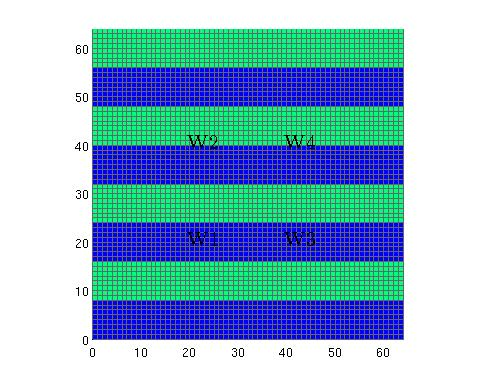
\includegraphics[width=4.3cm,height=4.3cm,keepaspectratio]{perm_he_1.jpg}
 \vspace{-20pt}
\caption{ Heterogeneous permeability, 4 wells.}\label{fig:hep}
\vspace{-15pt}
\end{wrapfigure}

\normalsize
As mentioned above, we studied flow through a porous medium with \emph{heterogeneous permeability} layers. A grid of
$nx = ny = 64$ elements is studied. We use 8 layers of the same size, 
4 layers with one value of permeability $\sigma_1$, followed by a layer with a different permeability value $\sigma_2$. Figure \ref{fig:hep} shows these layers. The permeability of one set of layers is set to $\sigma_1=1mD$, the permeability of the other set $\sigma_2$ is changed. 
Therefore, the contrast in permeability between the layers $(\frac{\sigma_2}{\sigma_1}=\sigma_2)$,
depends on the value of $\sigma_2$.\\
We investigate the dependence on the contrast in permeability value between the layers for the ICCG and DICCG methods.
The permeability  $\sigma_2$ varies from $\sigma_2=10^{-1}mD$ to $\sigma_2=10^{-3}mD$. 
 The tolerance is set as $10^{-11}$ for the snapshots as well as for the original problem.\\
\renewcommand{\arraystretch}{1.3}
\begin{table}[!ht]
\centering
\begin{minipage}{.65\textwidth}
\vspace{-20pt}
\centering
\begin{tabular}{ |c|c|c|c|} 
\hline
 $\kappa_2$ (mD) & $10^{-1}$& $10^{-2}$ & $10^{-3}$ \\
 \hline
  ICCG  & 75& 103&110\\ 
 
  DICCG  & 1 & 1& 1\\ 
 \hline
\end{tabular}
\caption{Table with the number of iterations for different contrasts in the permeability of the layers
for the ICCG and DICCG methods.}
\label{table:hei}\end{minipage}
\vspace{-10pt}
\end{table}

Table \ref{table:hei} shows the number of iterations required to achieve convergence 
for ICCG and DICCG for various permeability contrasts between the layers. \\
The plot of the residual and the solution 
to the problem are presented in Figures \ref{fig:convhe1} and \ref{fig:solhe1} for a value of permeability $\sigma_2=10^{-2}$.\\
In Table \ref{table:hei} we observe that the number of 
iterations increases when the contrast between the permeability layers increases for ICCG. For DICCG, 
we observe that we only need one iteration despite the change in permeability contrast between the layers.
\begin{figure}[!h]
\centering
\begin{minipage}{.4\textwidth}
 \centering
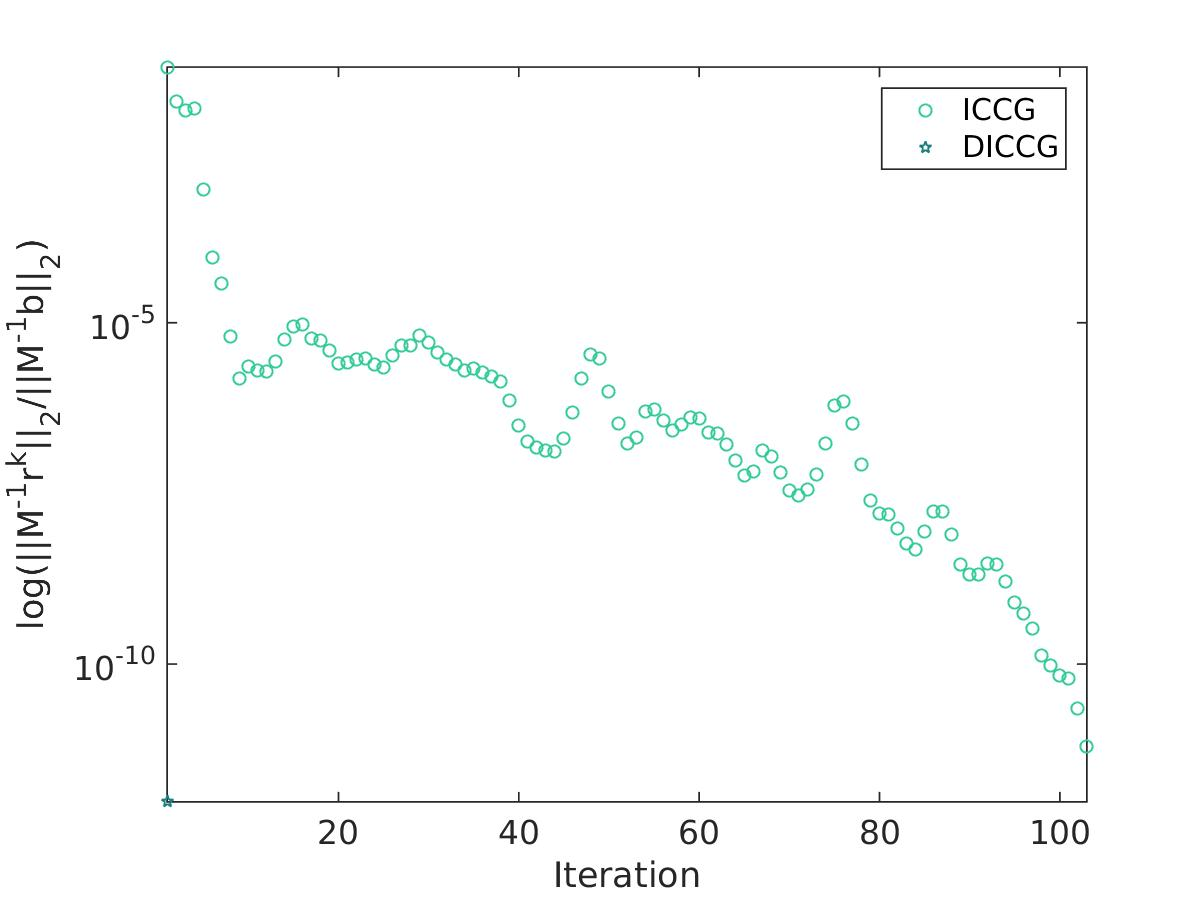
\includegraphics[width=5cm,height=5cm,keepaspectratio]
{conv_4w.jpg}
\caption{Convergence for the heterogeneous problem, 64 x 64 grid cells,  $\sigma_2=10^{-2}mD$.}
\label{fig:convhe1}
\end{minipage}%
\hspace{10pt}
\begin{minipage}{.4\textwidth} 
\centering 
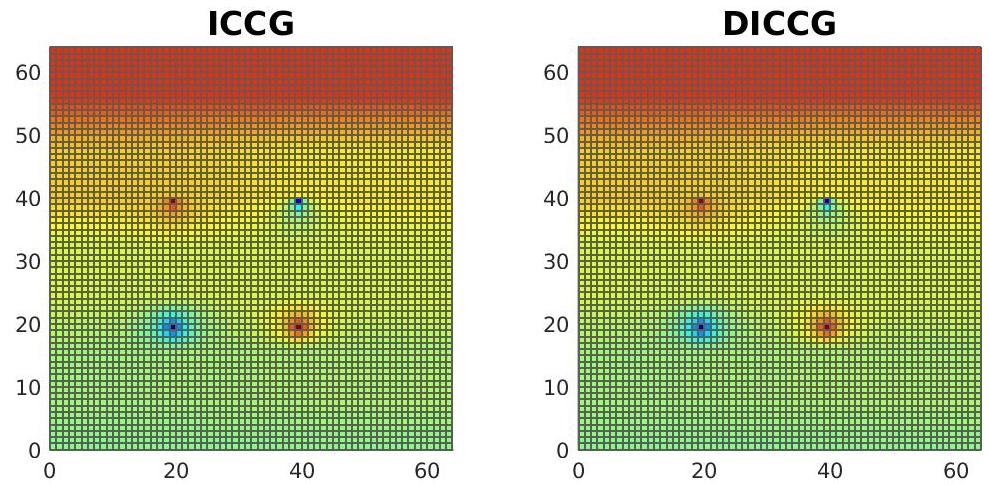
\includegraphics[width=6.5cm,height=6.5cm,keepaspectratio]
{sol_4w.jpg}
\caption{Solution of the heterogeneous problem, 64 x 64 grid cells, $\sigma_2=10^{-2}mD$.}
\label{fig:solhe1}
\end{minipage}
\end{figure}
%\begin{figure}[!h]
%\centering 
%\includegraphics[width=5cm,height=5cm,keepaspectratio]
%{perm_he_1.jpg}



\textbf{\emph{Case 2, Neumann boundary conditions everywhere.}}\\
In this case, four wells are positioned in the corners and have a bhp of -1 bar. One well
is positioned in the center of the domain and has a bhp of +4 bars
(see Figure \ref{fig:hep_2}). Homogeneous Neumann boundary conditions are posed on all boundaries. For this case, we use a set of four linearly independent snapshots as deflation vectors. We also use a linearly dependent set of 15 snapshots and the basis of POD (linearly independent set) obtained from the 15 snapshots. We set the same boundary conditions as in the original problem for all the snapshots.
The four linearly independent snapshots ($z_1-z_4$) are obtained giving a value of zero to one well and non-zero values to the other wells, such that the sum of the well pressures is equal to zero. The set of 15 snapshots are all the possible combinations of wells that satisfy that the flow in equals the flow out the reservoir.
A summary of the configurations is presented below.
\renewcommand{\arraystretch}{1.3}
\begin{table}[!ht]\centering
\begin{minipage}{.45\textwidth}
\vspace{-10pt}
\centering
\begin{tabular}{ |c|c|c|c|c|c|} 
 \hline
  \multicolumn{6}{|l|}{System configuration} \\ 
  \hline
  \multicolumn{6}{|c|}{Well pressures (bars)}\\
  \hline
  &W1 &W2 &W3 &W4 &W5 \\
  \hline
&-1 & -1& -1& -1& -1\\
\hline
\multicolumn{6}{|l|}{Snapshots (4 linearly independent)} \\
\hline
 &W1 &W2 &W3 &W4 &W5 \\
  \hline

$\mathbf{z}_1$& 0&-1 &-1 &-1 &3 \\
$\mathbf{z}_2$& -1&0 &-1 &-1 &3  \\
$\mathbf{z}_3$& -1&-1 &0 &-1 &3  \\
$\mathbf{z}_4$& -1&-1 &-1 &0 &3  \\
 \hline
 \end{tabular}
\label{table:case2}\end{minipage}%
\hspace{10pt}
 \begin{minipage}{.45\textwidth}
 \begin{tabular}{ |c|c|c|c|c|c|} 
 \hline
 \multicolumn{6}{|l|}{Snapshots (linearly dependent)} \\
\hline
 &W1 &W2 &W3 &W4 &W5 \\
  \hline
$\mathbf{z}_5$& -1&-1 &-1 &-1 &4  \\
$\mathbf{z}_6$& -1&0 &0 &-1 &2  \\
$\mathbf{z}_7$& -1&-1 &0 &0 &2  \\
$\mathbf{z}_8$& -1&0 &-1 &0 &2  \\
$\mathbf{z}_9$& 0&-1 &-1 &0 &2  \\
$\mathbf{z}_{10}$& 0&-1 &0 &-1 &2  \\
$\mathbf{z}_{11}$& 0&0 &-1 &-1 &2  \\
$\mathbf{z}_{12}$& -1&0 &0 &0 &1  \\
$\mathbf{z}_{13}$& 0&-1 &0 &0 &1  \\
$\mathbf{z}_{14}$& 0&0 &-1 &0 &1  \\
$\mathbf{z}_{15}$& 0&0 &0 &-1 &1  \\
 \hline
 \end{tabular}

\label{table:case2}\end{minipage}\caption{Table with the well configuration of the system and the snapshots used for the Case 2, we use homogeneous Neumann boundary conditions.}
\vspace{-10pt}
\end{table}

\normalsize

\emph{Heterogeneous permeability layers}\\

\begin{wrapfigure}{R}{4.3cm}
\centering 
\vspace{-10pt}
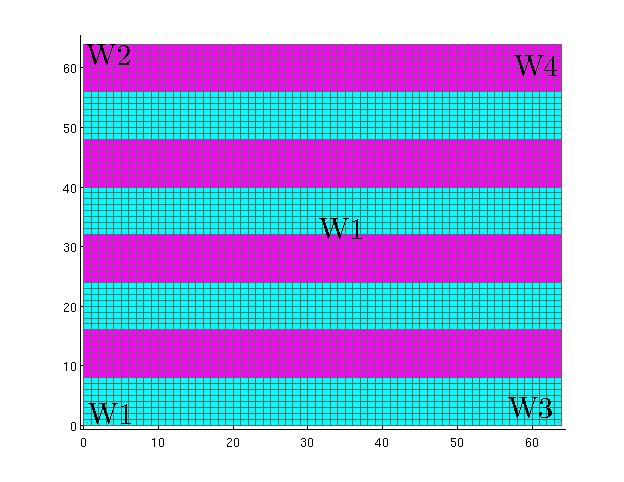
\includegraphics[width=4.3cm,height=4.3cm,keepaspectratio]{perm_he_2.jpg}
 \vspace{-25pt}
\caption{ Heterogeneous permeability, 5 wells.}\label{fig:hep_2}
\vspace{-15pt}
\end{wrapfigure} 
As in the previous case, single-phase flow through a porous medium with heterogeneous permeability layers is studied.
A grid of $nx = ny = 64$ elements is investigated. The deflation vectors used in this case are the 4 snapshots ($\mathbf{z}_1$-$\mathbf{z}_4$), a set of 15 linearly dependent vectors and 4 basis vectors obtained for the POD method from the latter set.\\
The snapshots and the solutions are obtained with a tolerance of $10^{-11}$. \\
\begin{figure}[!ht]
%\begin{wrapfigure}{R}{5cm}
%\vspace{-20pt}
 \centering
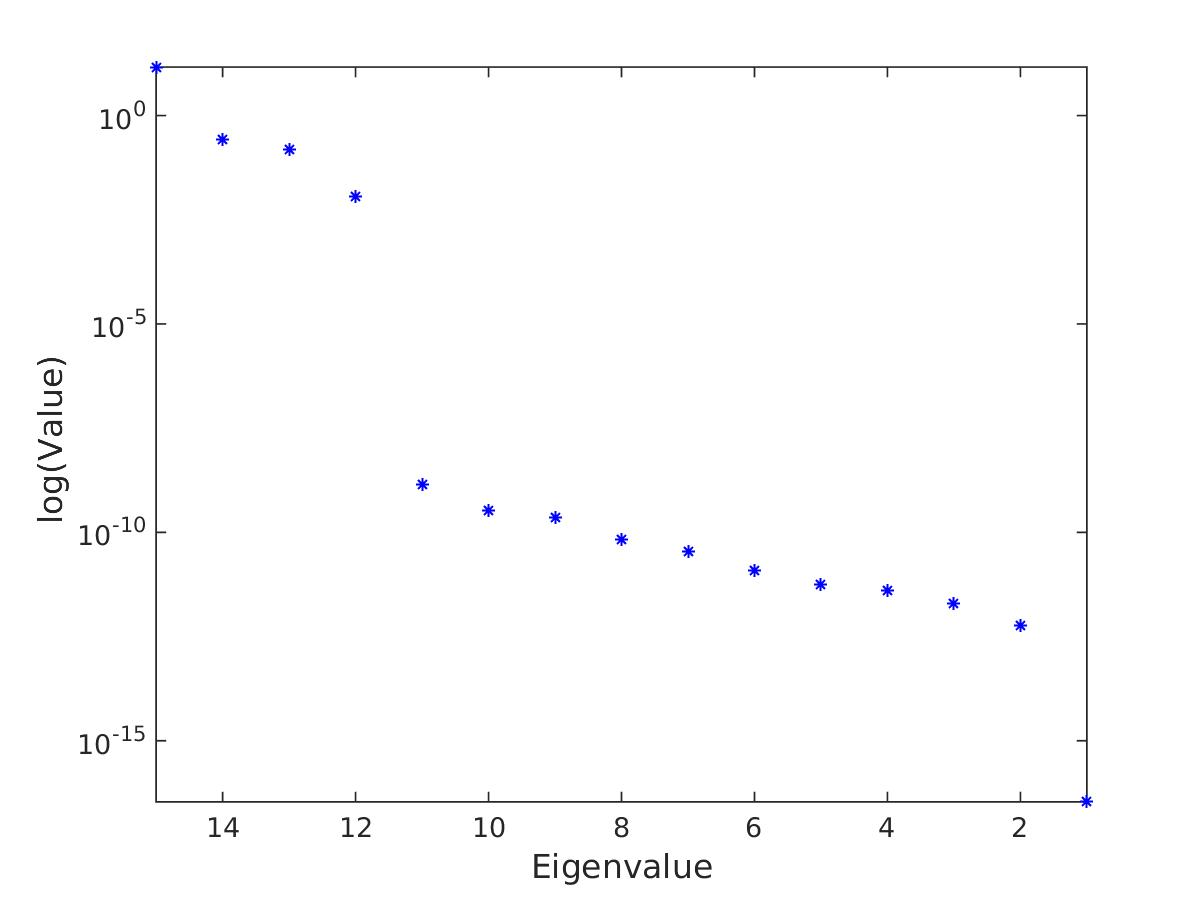
\includegraphics[width=7cm,height=7cm,keepaspectratio]
{eig_pod_5w.jpg}
%\vspace{-10pt}
\caption{Eigenvalues of the snapshot correlation matrix $\mathbf{R}=\mathbf{X}\mathbf{X}^T$, 15 snapshots used.}
%\vspace{-20pt}
\label{fig:eig}
%\end{wrapfigure}
\end{figure} 
Table \ref{table:he22} shows the number of iterations required to reach convergence for ICCG method and the deflation method with four linearly independent snapshots as deflation vectors DICCG$_{4}$, 15 linearly dependent snapshots DICCG$_{15}$ and the basis vectors of POD, DICC$G_{POD}$\footnote{The * means that the solution is not reached.}. 
For the deflation vectors of DICCG$_{POD}$ we plot the eigenvalues of the snapshot correlation matrix $\mathbf{R}=\mathbf{X}^T \mathbf{X}$ (see section \ref{POD}) in Figure \ref{fig:eig}. We observe that there are 4 eigenvalues much larger than the rest of the eigenvalues which are responsible for the diconvergence of the method. In DICCG$_{POD}$ we use the eigenvectors corresponding to the larger eigenvalues as deflation vectors.\\
The plot of the residual and the solution of the problem are presented in
Figure \ref{fig:convhe2} and \ref{fig:solhe2} for the ICCG and DICCG methods for the case of $\sigma_2=10^{-1}$.\\
\renewcommand{\arraystretch}{1.3}
\begin{table}[!ht]\centering
\begin{minipage}{.8\textwidth}
\vspace{-10pt}
\centering
\begin{tabular}{ |c|c|c|c|} 
\hline
 $\sigma_2$ (mD) & $10^{-1}$& $10^{-2}$ & $10^{-3}$ \\
 \hline
  ICCG  & 90& 115&131\\ 
 
  DICCG$_4$  & 1 & 1& 1\\ 
  DICCG$_{15}$  & 200* & 200*& 200*\\
  DICCG$_{POD}$  & 1 & 1& 1\\
 \hline
\end{tabular}
\caption{Table with the number of iterations for different contrast in the permeability of the layers
for the ICCG, DICCG$_4$, DICCG$_{15}$, and DICCG$_{POD}$ methods, tolerance of solvers and snapshots $10^{-11}$.}
\label{table:he22}\end{minipage}
\vspace{-10pt}
\end{table}

In Table \ref{table:he22}, for the ICCG method, we observe that the number of iterations 
increases if the contrast in the permeability increases. For the DICCG method with 4 linearly independent deflation vectors and 4 basis vectors of POD, convergence is reached 
within one iteration. However, for the case of 15 linearly dependent vectors, the solution is not reached within the 200 iterations allowed for this problem.\\

\vspace{-5mm}
\begin{figure}[!h]
\centering
\begin{minipage}{.4\textwidth}
 \centering
\includegraphics[width=6.5cm,height=6.5cm,keepaspectratio]
{/mnt/sda2/cortes/Results/16_09/article_sp/size_64perm_1_5wells11/conv_deftol-11.jpg}
\caption{Convergence for the heterogeneous problem, 64 x 64 grid cells, $\sigma_2=10^{-1}$.}
\label{fig:convhe2}
\end{minipage}%
\hspace{10 pt}
\begin{minipage}{.4\textwidth}
 \centering
 %\vspace{-2cm}
\includegraphics[width=6cm,height=6cm,keepaspectratio]
{/mnt/sda2/cortes/Results/16_09/article_sp/size_64perm_1_5wells11/solution.jpg}
\vspace{0cm}
\caption{Solution of the heterogeneous problem, 64 x 64 grid cells, $\sigma_2=10^{-1}$.}
\label{fig:solhe2}
\end{minipage}
\end{figure}

\newpage
\emph{SPE 10 model}\\
This model has large variations in the permeability coefficients, the contrast between coefficients is of the order of $ 10^7$.
It has 5 sources or wells, four producers in the corners (negative) and one injector in the center (positive).
The model contains 60 x 220 x 85 cells. We study the dependence of the ICCG and the DICCG method on the size of the problem. One layer is studied with various grid sizes 16 x 56, 30 x 110, 46 x 166 and 60 x 220, and the complete model containing 85 layers.
Permeability is upscaled
averaging the permeability in each grid using the harmonic-arithmetic average algorithm from MRST.
The permeability of the coarser grid (16 x 56 cells) is shown in Figure \ref{fig:permc} and the complete model in Figure \ref{fig:permcc}.
The permeability contrast for the diverse grid size problems is shown in Table \ref{table:permgs}. From this table, we observe that the contrast in the permeability for different grid sizes varies slightly, but that the order
of magnitude remains the same for all the cases.\\
Snapshots are obtained solving the system with different well
configurations (\emph{Configuration 2}). As before, we simulate single-phase incompressible flow.\\
The system and snapshots are solved with an accuracy of $10^{-7}$.
In the first experiment with the deflation method, the four linearly independent snapshots are used as deflation vectors (DICCG). Then, 
15 linearly dependent vectors and finally 4 vectors of the POD basis are used as deflation vectors (DICCG$_{POD}$). \\ 
\begin{figure}[!h]
\centering
\begin{minipage}{.4\textwidth}
 \centering
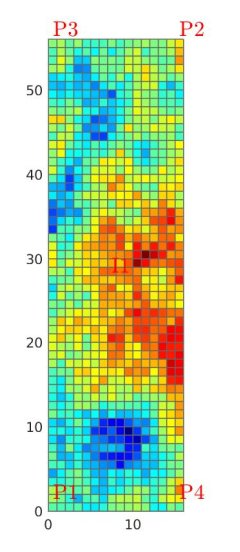
\includegraphics[width=4.5cm,height=4.5cm,keepaspectratio]
{perm_layer_2.jpg}
\caption{SPE 10 benchmark, 2nd layer 16 x 56 grid cells, permeability field.}
\label{fig:permc}
\end{minipage}%
\hspace{4mm}
\begin{minipage}{.4\textwidth}
 \centering
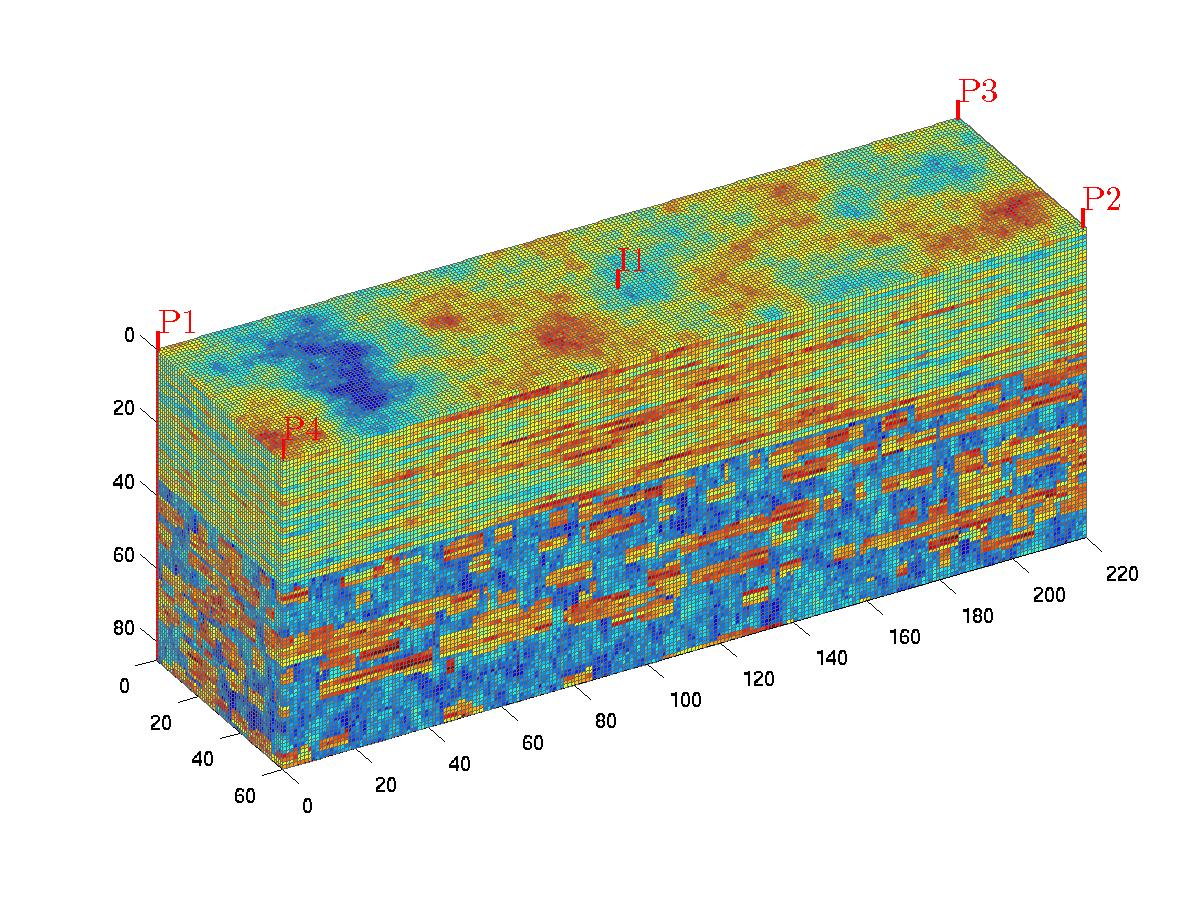
\includegraphics[width=5.5cm,height=5.5cm,keepaspectratio]
{perm_layer_.jpg}
\caption{SPE 10 benchmark, permeability field.}
\label{fig:permcc}
\end{minipage}
\end{figure}


\begin{table}[!ht]
\centering
\begin{tabular}{ |c|c|c|c|c|c|  } 
 \hline
  Grid size & 16x56x1& 30x110x1& 46x166x1& 60x220x1&60x220x85\\
  \hline
  Contrast ($\times10^{7}$) & 1.04 & 2.52&  2.6&  2.8 &3\\ 
\hline
\end{tabular}
\caption{Table with the number of iterations for different grid sizes
for the ICCG, DICCG$_4$, DICCG$_{15}$, and DICCG$_{POD}$ methods, tolerance of solvers and snapshots $10^{-11}$.}
\label{table:permgs}
\end{table}

The number of iterations required to achieve convergence with the ICCG and DICCG methods for various
grid sizes is presented in Table \ref{table:itgrid}. \\
The convergence and the solution obtained with the ICCG and DICCG methods are presented in Figure \ref{fig:convspe85} and Figure \ref{fig:solspe} for the complete problem. 
In Table \ref{table:permgs} we observe that for the ICCG method the required iterations to reach convergence increases as the size of the grid increases. Meanwhile, for the deflated methods only few iteration are required and it does not depend on the size of the grid. According to theory, the number of iterations should be 1 for this cases, but due to the large contrast between permeability coefficients, the required tolerance to achieve the solution within one iteration can be larger. Therefore, the approximation with the desired accuracy cannot be achieved within one iteration (see Section \ref{as}). However, we observe in Figure \ref{fig:convspe85} that the first iteration has a relative residual smaller than $10^{-10}$ for the DICCG$_4$ and DICCG$_{POD}$ methods.
We also observe that for the deflated method with 15 linearly dependent snapshots as deflation vectors (DICCG$_{15}$), the relative residual is close to $10^{-7}$ for the first time steps, and then it increases, which shows that is not very stable. 

\begin{table}[!ht]
\centering
\begin{tabular}{|c |c|c|c|c|c| c| } 
 \hline
Method  & 16x56x1& 30x110x1& 46x166x1& 60x220x1&60x220x85\\
   \hline
  ICCG & 45 & 101&  178 &  219&1011 \\ 
   DICCG$_{15}$ & 500* & 500*&  500* &  500*& 2000*\\ 
   DICCG$_{4}$ & 1 & 2&  3 &  2& 2\\  
   DICCG$_{POD}$ & 1 & 2&  3 &  2 &2\\ 
\hline
\end{tabular}
\caption{Table with the number of iterations for ICCG and DICCG methods, 
various grid sizes.}
\label{table:itgrid}
\end{table}

\begin{figure}[!h]
\centering
\begin{minipage}{.5\textwidth}
 \centering
\includegraphics[width=7cm,height=7cm,keepaspectratio]
{/mnt/sda2/cortes/Results/16_09/article_sp/SPE10_85layers_5w_tol-11/conv_deftol-11.jpg}
\caption{Convergence for the SPE 10 benchmark, 60 x 220 x 85 grid cells, accuracy of the snapshots and solvers $10 ^{-11}$.}
\label{fig:convspe85}
\end{minipage}%
\hspace{3mm}
\begin{minipage}{.45\textwidth}
 \centering
\includegraphics[width=6cm,height=6cm,keepaspectratio]
{/mnt/sda2/cortes/Results/16_09/article_sp/SPE10_85layers_5w_tol-11/solution.jpg}
\vspace{.7cm}
\caption{Solution of the SPE 10 benchmark, 60 x 220 x 85 grid cells, accuracy of the snapshots and solvers $10 ^{-11}$.}
\label{fig:solspe}
\end{minipage}
\end{figure}
\newpage

\newpage
\newpage
\subsection{Compressible Problem}
\emph{\textbf{Model parameters}}\\

In this section we model single-phase flow through a porous medium for a case when the density depends on the pressure according to Equation \ref{eq:rhoeq}. We solve Equation \eqref{eq:ce6} for a fluid with the following characteristics:
\begin{itemize}
 \item $\mu = 1 cp$,
 \item $\rho = 1014 kg/m^3$,
\end{itemize}
In the compressible case, the compressibility of the fluid is:
\begin{itemize}
 \item $c= 1 \times 10^{-3}$.
\end{itemize}
Equation \eqref{eq:ce6} is non-linear due to the dependence of the density on the pressure. Therefore, we need to linearize this equation via the Newton-Raphson method and solve the resulting linear system. After linearization we obtain the linear system \eqref{eq:lsJ} and we solve it with an iterative method, a summary of the procedure is presented in Table \ref{table:solstages}. The resulting linear system is solved with ICCG and DICCG methods. We compute the solution of the system for the first 10 time steps with the ICCG method. The rest of the time steps is solved with DICCG. The previously computed solutions are used as snapshots. Ten POD basis vectors are obtained from the $11^{th}$ time step on using all teh previously computed snapshots. \\
\begin{wrapfigure}{R}{5cm}
\centering 
\vspace{-20pt}
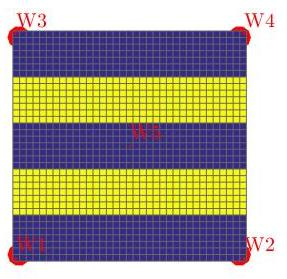
\includegraphics[width=5cm,height=5cm,keepaspectratio]{perm_comp.jpg}
 \vspace{-15pt}
\caption{ Heterogeneous permeability, 5 wells, compressible problem.}\label{fig:pc}
\vspace{-10pt}
\end{wrapfigure} 

We study an academic layered problem that consists of layers with two different permeability values (see Figure \ref{fig:pc}). The first layer has a permeability of $\sigma_1 = 30mD$, and the permeability of the second layer is varied $\sigma_2 =$ [3mD, 0.3mD, 0.03mD]. Therefore, the contrast between the layers is $10^{-1},$ $10^{-2}$ and $10^{-3}$.
The domain is a square with five wells, Four of which are positioned in the corners of the domain and one well is placed in the center. The size of the grid and the length of the domain are changed in such a way that the length of a grid cell is 1 m. The length of the domain is 35, 70 and 105 m. We use homogeneous Neumann boundary conditions in all the boundaries. \\
The initial pressure of the reservoir is set as 200 bars. The pressure in the corner wells is 100 bars and in the central well is 600 bars.  A summary of the well configuration is presented in Table \ref{table:ccase1}.

 \renewcommand{\arraystretch}{1.3}
\begin{table}[!ht]\centering
\begin{minipage}{.7\textwidth}
\vspace{-10pt}
\centering
\begin{tabular}{ |c|c|c|c|c|c|} 
 \hline
  \multicolumn{6}{|l|}{System configuration} \\ 
  \hline
  \multicolumn{6}{|c|}{Well pressures (bars)}\\
  \hline
  &W1 &W2 &W3 &W4 &W5 \\
  \hline
&100 & 100& 100& 100& 600\\
\hline
\multicolumn{6}{|l|}{Snapshots } \\
  \hline
$\mathbf{z}_1$&200 & 100& 100& 100& 500\\
$\mathbf{z}_2$&100 & 200& 100& 100& 500\\
$\mathbf{z}_3$&100 & 100& 200& 100& 500\\
$\mathbf{z}_4$&100 & 100& 100& 200& 500\\
 \hline
 \end{tabular}
\caption{Table with the well configuration of the system and the snapshots used for the compressible problem Case 1, we use homogeneous Neumann boundary conditions.}\label{table:ccase1}
\end{minipage}
\end{table}
 
The simulation was performed during 152 days with 52 time steps and a time step of 3 days. The tolerance of the NR method and the linear solvers is $10^{-5}$.\\
\newpage
\textbf{Different contrast in permeability.}\\
As mentioned previously we change the contrast between the permeability layers, in this section we present the results obtained for three different contrast with a grid of $35 \times 35$ grid cells.

\textbf{Contrast between permeability layers of $10^{-1}$.}\\
In Figure \ref{fig:compsol_1}, the solution obtained with the ICCG method is presented, the solution is the same for all methods. The upper left figure represents the pressure field at the final time step. The upper right figure represents the pressure across the diagonal joining the (0,0) and (35,35) grid cells for all the time steps. We observe the initial pressure (200 bars) in this diagonal and the evolution of the pressure field through time. In the lower figure, we observe the surface volume rate for the five wells during the simulation.


\begin{figure}[!h]
\centering
\begin{minipage}{.7\textwidth}
 \centering
\includegraphics[width=8cm,height=8cm,keepaspectratio]
{/home/wagm/cortes/Localdisk/Results/sp_article/size_35perm_1_5wells_c_1e-3_s_52upd/solution.jpg}
\caption{Solution of the compressible problem solved with the ICCG method.}
\label{fig:compsol_1}
\end{minipage}
\end{figure}


As mentioned before, the deflation vectors used for the DICCG method are the basis vectors of POD, these basis vectors are the eigenvectors corresponding of the largest eigenvalues of the snapshot correlation matrix $\mathbf{X}$. The snapshot correlation matrix is constructed with the previously computed solutions, i.e., the solutions of the previous time steps. The eigenvalues of the snapshot correlation matrix $\mathbf{R}=\frac{1}{m}\mathbf{X}\mathbf{X}^T$ for the 50$^{th}$ time step are presented in Figure \ref{fig:eig_POD_1}. 
\begin{figure}[!h]
\centering
\begin{minipage}{.4\textwidth}
 \centering
 \vspace{-3mm}
\includegraphics[width=6cm,height=6cm,keepaspectratio]{/home/wagm/cortes/Localdisk/Results/sp_article/size_35perm_1_5wells_c_1e-3_s_52upddv_10pod/eigs/eigs1stepA.jpg}
 \vspace{-10pt}
\caption{Eigenvalues of the original matrix $\mathbf{J}$, time step 1.}\label{fig:eigs_A_1}
\end{minipage}%
\hspace{1cm}
\begin{minipage}{.4\textwidth}
 \centering
 %\vspace{-5mm}
\includegraphics[width=6cm,height=6cm,keepaspectratio]{/home/wagm/cortes/Localdisk/Results/sp_article/size_35perm_1_5wells_c_1e-3_s_52upddv_10pod/eig_pod50.jpg}
\vspace{-5mm}
\caption{Eigenvalues of the data snapshot correlation matrix $\mathbf{R}=\mathbf{X}\mathbf{X}^T$, time step 50.}
\label{fig:eig_POD_1}
\end{minipage}
\end{figure}

For this case, only the first time step requires more than two NR iterations. Therefore, we solely study the behavior of the linear solvers during the first two NR iterations. The number of iterations necessary to reach convergence with the linear solvers is presented for the first two NR iterations in Figure \ref{fig:NR_IC_1} for the ICCG method, Figure \ref{fig:NR_D10_1} for the deflated method DICCG using 10 POD basis vectors as deflation vectors.
The eigenvalues of the matrices are presented in Figure \ref{fig:eigs_A_1} for the original system matrix $\mathbf{J}$ for the first time step, Figure \ref{fig:eigs_MA_1} for the preconditioned system and Figure \ref{fig:eigs_PA_1} the deflated system DICCG. \\
%The eigenvalues of the covariance matrix  $\bar{\mathbf{R}}=\frac{1}{m}\sum_{i=1}^{m}(\mathbf{z}_i-\mathbf{z})(\mathbf{z}_i-\mathbf{z})^T$ are presented in Figure \ref{fig:eig_PODr}.\\

\begin{figure}[!h]
\centering
\begin{minipage}{.4\textwidth}
\vspace{-0.9cm}
\hspace{-1cm}
\includegraphics[width=8cm,height=8cm,keepaspectratio]
{/home/wagm/cortes/Localdisk/Results/sp_article/size_35perm_1_5wells_c_1e-3_s_52upd/iterations_4NR.jpg}
\vspace{-1.3cm}
\caption{Number of iterations of the ICCG method for the first two NR iterations.}
\label{fig:NR_IC_1}
\end{minipage}%
\hspace{15mm}
\begin{minipage}{.4\textwidth}
 \centering
 \vspace{-5mm}
\includegraphics[width=6cm,height=6cm,keepaspectratio]
{/home/wagm/cortes/Localdisk/Results/sp_article/size_35perm_1_5wells_c_1e-3_s_52upddv_10pod/eigs/eigs1step.jpg}
\caption{Eigenvalues of the preconditioned matrix, time step 1.}
\label{fig:eigs_MA_1}
\end{minipage}
\end{figure}

\begin{figure}[!h]
\centering
\begin{minipage}{.4\textwidth}
\vspace{-0.4cm}
\hspace{-1cm}
\includegraphics[width=8cm,height=8cm,keepaspectratio]
{/home/wagm/cortes/Localdisk/Results/sp_article/size_35perm_1_5wells_c_1e-3_s_52upddv_10pod/iterations_4NR.jpg}
\vspace{-1.3cm}
\caption{Number of iterations of the DICCG method for the first two NR iterations.}
\label{fig:NR_D10_1}
\end{minipage}%
\hspace{15mm}
\begin{minipage}{.4\textwidth}
 \centering
\includegraphics[width=6cm,height=6cm,keepaspectratio]
{/home/wagm/cortes/Localdisk/Results/sp_article/size_35perm_1_5wells_c_1e-3_s_52upddv_10pod/eigs/eigsPA11step.jpg}
\caption{Eigenvalues of the deflated system DICCG with 10 deflation vectors.}
\label{fig:eigs_PA_1}
\end{minipage}
\end{figure}
\newpage
From Figure \ref{fig:eigs_MA_1} and Figure \ref{fig:eigs_PA_1} we observe that the smallest eigenvalues are removed from the system, which implies that the condition number is reduced. From the spectrum of these systems, we observe that after the deflation procedure we reduce in one order of magnitude the condition number (see Table \ref{table:cn_1}). \\
\begin{table}[!ht]\centering
\begin{minipage}{.7\textwidth}
\vspace{-10pt}
\centering
\begin{tabular}{ |c|c|c|c|} 
  \hline
 Matrix &$\lambda_{max}$ &$\lambda_{min}$ &$\kappa_2=\frac{\lambda_{max}}{\lambda_{min}}$  \\
  \hline
$\mathbf{M}^{-1}\mathbf{J}$ &1 & $\approx 10^{-2}$&$\approx 10^2$\\
$\mathbf{P}\mathbf{M}^{-1}\mathbf{J}$ &1 & $\approx 10^{-1}$&$\approx 10^1$\\
 \hline
 \end{tabular}
\caption{Condition number of the preconditioned and deflated systems.}\label{table:cn_1}
\end{minipage}
\end{table}

From Figure \ref{fig:NR_IC_1} and Figure \ref{fig:NR_D10_1}, we observe that the reduction of the condition number results in a reduction of the number of iterations for the first and second NR iterations of the deflated method (DICCG) compared with the ICCG method. For the ICCG method, we need in average 28 linear iterations in the first two NR iterations to reach the desired tolerance. In contrast, for the deflated method DICCG, we need in average 1 iteration for the first NR iteration and only three more NR iterations with an average of 9 linear iterations after the 10 snapshots are computed for the second NR iteration. A summary is presented in Table \ref{table:liter}.\\

 
\textbf{Contrast between permeability layers of $10^{-2}$.}\\
The solution obtained with the ICCG method is presented in Figure \ref{fig:compsol_2}, the solution is the same for the DICCG method. The eigenvalues of the snapshot correlation matrix $\mathbf{R}$ for the 50$^{th}$ time step are presented in Figure \ref{fig:eig_POD_2}. 
We can observe in this figure that there are 16 eigenvalues of the correlation matrix that are larger than the rest. Therefore, the largest amount of information might be contained in these vectors. 

\begin{figure}[!h]
\centering
\begin{minipage}{.7\textwidth}
 \centering
\includegraphics[width=8cm,height=8cm,keepaspectratio]
{/home/wagm/cortes/Localdisk/Results/sp_article/size_35perm_2_5wells_c_1e-3_s_52upd/solution.jpg}
\caption{Solution of the compressible problem solved with the ICCG method.}
\label{fig:compsol_2}
\end{minipage}
\end{figure}

\begin{figure}[!h]
\centering
\begin{minipage}{.4\textwidth}
 \centering
 \vspace{-3mm}
\includegraphics[width=6cm,height=6cm,keepaspectratio]{/home/wagm/cortes/Localdisk/Results/sp_article/size_35perm_2_5wells_c_1e-3_s_52upddv_10pod/eigs/eigs1stepA.jpg}
 \vspace{-10pt}
\caption{Eigenvalues of the original matrix $\mathbf{J}$, time step 1.}\label{fig:eigs_A_2}
\end{minipage}%
\hspace{1cm}
\begin{minipage}{.4\textwidth}
 \centering
 %\vspace{-5mm}
\includegraphics[width=6cm,height=6cm,keepaspectratio]{/home/wagm/cortes/Localdisk/Results/sp_article/size_35perm_2_5wells_c_1e-3_s_52upddv_10pod/eig_pod50.jpg}
\vspace{-5mm}
\caption{Eigenvalues of the data snapshot correlation matrix $\mathbf{R}=\mathbf{X}\mathbf{X}^T$, time step 50.}
\label{fig:eig_POD_2}
\end{minipage}
\end{figure}

Only the first time step requires more than two NR iterations. Therefore, we solely study the behavior of the linear solvers during the first two NR iterations. The number of iterations necessary to reach convergence with the linear solvers is presented for the first two NR iterations in Figure \ref{fig:NR_IC_2} for the ICCG method, Figure \ref{fig:NR_D10_2} for the deflated method DICCG using 10 POD basis vectors as deflation vectors.
The eigenvalues of the matrices are presented in Figure \ref{fig:eigs_A_2} for the original system matrix $\mathbf{J}$ for the first time step, Figure \ref{fig:eigs_MA_2} for the preconditioned system and Figure \ref{fig:eigs_PA_2} the deflated system DICCG. For the deflated system the first 10 eigenvalues are very small and the scale used for the preconditioned and deflated method is the same, therefore, they are not visible in this figure. \\

\begin{figure}[!h]
\centering
\begin{minipage}{.4\textwidth}
\vspace{-0.9cm}
\hspace{-1cm}
\includegraphics[width=8cm,height=8cm,keepaspectratio]
{/home/wagm/cortes/Localdisk/Results/sp_article/size_35perm_2_5wells_c_1e-3_s_52upd/iterations_4NR.jpg}
\vspace{-1.3cm}
\caption{Number of iterations of the ICCG method for the first two NR iterations.}
\label{fig:NR_IC_2}
\end{minipage}%
\hspace{15mm}
\begin{minipage}{.4\textwidth}
 \centering
 \vspace{-5mm}
\includegraphics[width=6cm,height=6cm,keepaspectratio]
{/home/wagm/cortes/Localdisk/Results/sp_article/size_35perm_2_5wells_c_1e-3_s_52upddv_10pod/eigs/eigs1step.jpg}
\caption{Eigenvalues of the preconditioned matrix, time step 1.}
\label{fig:eigs_MA_2}
\end{minipage}
\end{figure}

\begin{figure}[!h]
\centering
\begin{minipage}{.4\textwidth}
\vspace{-0.4cm}
\hspace{-1cm}
\includegraphics[width=8cm,height=8cm,keepaspectratio]
{/home/wagm/cortes/Localdisk/Results/sp_article/size_35perm_2_5wells_c_1e-3_s_52upddv_10pod/iterations_4NR.jpg}
\vspace{-1.3cm}
\caption{Number of iterations of the DICCG method for the first two NR iterations.}
\label{fig:NR_D10_2}
\end{minipage}%
\hspace{15mm}
\begin{minipage}{.4\textwidth}
 \centering
\includegraphics[width=6cm,height=6cm,keepaspectratio]
{/home/wagm/cortes/Localdisk/Results/sp_article/size_35perm_2_5wells_c_1e-3_s_52upddv_10pod/eigs/eigsPA11step.jpg}
\caption{Eigenvalues of the deflated system DICCG with 10 deflation vectors.}
\label{fig:eigs_PA_2}
\end{minipage}
\end{figure}
\newpage

From Figure \ref{fig:NR_IC_2} and Figure \ref{fig:NR_D10_2}, we observe that the number of iterations for the first and second NR iterations is lower for the deflated methods compared with the ICCG method. For the ICCG method, we need in average 19 and 21 linear iterations in the first two NR iterations to reach the desired accuracy. In contrast, for the deflated method DICCG, we need in average 10 iterations for the first NR iteration and 14 iterations in average for the second NR iteration (see Table \ref{table:liter}). \\
\textbf{16 deflation vectors}\\
As mentioned previously, there are 16 eigenvalues of the snapshot correlation matrix that are larger than the rest, therefore we perform the same experiments as before with 16 deflation vectors (the eigenvectors corresponding to the 16 largest eigenvalues).
As in the previous case, only two NR iterations are studied. The number of iterations necessary to achieve convergence with the deflated method DICCG using 16 POD basis vectors as deflation vectors  is presented in Figure \ref{fig:NR_D16_2}.
The eigenvalues of the preconditioned matrix are presented Figure \ref{fig:eigs_PA16_2} for the deflated system DICCG with 16 deflation vectors. \\

\begin{figure}[!h]
\centering
\begin{minipage}{.4\textwidth}
\vspace{-0.4cm}
\hspace{-1cm}
\includegraphics[width=8cm,height=8cm,keepaspectratio]
{/home/wagm/cortes/Localdisk/Results/sp_article/size_35perm_2_5wells_c_1e-3_s_52upddv_16pod/iterations_4NR.jpg}
\vspace{-1.3cm}
\caption{Number of iterations of the DICCG method for the first two NR iterations.}
\label{fig:NR_D16_2}
\end{minipage}%
\hspace{15mm}
\begin{minipage}{.4\textwidth}
 \centering
\includegraphics[width=6cm,height=6cm,keepaspectratio]
{/home/wagm/cortes/Localdisk/Results/sp_article/size_35perm_2_5wells_c_1e-3_s_52upddv_16pod/eigs/eigsPA17step.jpg}
\caption{Eigenvalues of the deflated system DICCG with 16 deflation vectors.}
\label{fig:eigs_PA16_2}
\end{minipage}
\end{figure}
\newpage

From Figure \ref{fig:NR_D16_2}, we observe that the number of iterations for the first NR iteration is reduced to one iteration, in average. For the second NR iteration, we need to compute the solution only for four time steps after the computation of the 16 snapshots, and the average number of linear iterations of these time steps is 12 (see Table \ref{table:liter}). Therefore, we can see that the optimal number of deflation vectors needed to obtain the largest reduction in the number of linear iterations is 16.\\




\textbf{Contrast between permeability layers of $10^{-3}$.}\\
The solution obtained with the ICCG method is presented in Figure \ref{fig:compsol_3}, the solution is the same for the DICCG method. The eigenvalues of the snapshot correlation matrix $\mathbf{R}$ for the 50$^{th}$ time step are presented in Figure \ref{fig:eig_POD_3}. 


\begin{figure}[!h]
\centering
\begin{minipage}{.7\textwidth}
 \centering
\includegraphics[width=8cm,height=8cm,keepaspectratio]
{/home/wagm/cortes/Localdisk/Results/sp_article/size_35perm_3_5wells_c_1e-3_s_52upd/solution.jpg}
\caption{Solution of the compressible problem solved with the ICCG method.}
\label{fig:compsol_3}
\end{minipage}
\end{figure}

\begin{figure}[!h]
\centering
\begin{minipage}{.4\textwidth}
 \centering
 \vspace{-3mm}
\includegraphics[width=6cm,height=6cm,keepaspectratio]{/home/wagm/cortes/Localdisk/Results/sp_article/size_35perm_3_5wells_c_1e-3_s_52upddv_10pod/eigs/eigs1stepA.jpg}
 \vspace{-10pt}
\caption{Eigenvalues of the original matrix $\mathbf{J}$, time step 1.}\label{fig:eigs_A_3}
\end{minipage}%
\hspace{1cm}
\begin{minipage}{.4\textwidth}
 \centering
 %\vspace{-5mm}
\includegraphics[width=6cm,height=6cm,keepaspectratio]{/home/wagm/cortes/Localdisk/Results/sp_article/size_35perm_3_5wells_c_1e-3_s_52upddv_10pod/eig_pod50.jpg}
%\vspace{-5mm}
\caption{Eigenvalues of the data snapshot correlation matrix $\mathbf{R}=\mathbf{X}\mathbf{X}^T$, time step 50.}
\label{fig:eig_POD_3}
\end{minipage}
\end{figure}

From Figure For this case, only the first time step requires more than two NR iterations. Therefore, we solely study the behavior of the linear solvers during the first two NR iterations. The number of iterations necessary to reach convergence with the linear solvers is presented for the first two NR iterations in Figure \ref{fig:NR_IC_3} for the ICCG method, Figure \ref{fig:NR_D10_3} for the deflated method DICCG using 10 POD basis vectors as deflation vectors.
The eigenvalues of the matrices are presented in Figure \ref{fig:eigs_A_3} for the original system matrix $\mathbf{J}$ for the first time step, Figure \ref{fig:eigs_MA_3} for the preconditioned system and Figure \ref{fig:eigs_PA_3} the deflated system DICCG. \\


\begin{figure}[!h]
\centering
\begin{minipage}{.4\textwidth}
\vspace{-0.9cm}
\hspace{-1cm}
\includegraphics[width=8cm,height=8cm,keepaspectratio]
{/home/wagm/cortes/Localdisk/Results/sp_article/size_35perm_3_5wells_c_1e-3_s_52upd/iterations_4NR.jpg}
\vspace{-1.3cm}
\caption{Number of iterations of the ICCG method for the first two NR iterations.}
\label{fig:NR_IC_3}
\end{minipage}%
\hspace{15mm}
\begin{minipage}{.4\textwidth}
 \centering
 \vspace{-5mm}
\includegraphics[width=6cm,height=6cm,keepaspectratio]
{/home/wagm/cortes/Localdisk/Results/sp_article/size_35perm_3_5wells_c_1e-3_s_52upddv_10pod/eigs/eigs1step.jpg}
\caption{Eigenvalues of the preconditioned matrix, time step 11.}
\label{fig:eigs_MA_3}
\end{minipage}
\end{figure}

\begin{figure}[!h]
\centering
\begin{minipage}{.4\textwidth}
\vspace{-0.4cm}
\hspace{-1cm}
\includegraphics[width=8cm,height=8cm,keepaspectratio]
{/home/wagm/cortes/Localdisk/Results/sp_article/size_35perm_3_5wells_c_1e-3_s_52upddv_10pod/iterations_4NR.jpg}
\vspace{-1.3cm}
\caption{Number of iterations of the DICCG method for the first two NR iterations.}
\label{fig:NR_D10_3}
\end{minipage}%
\hspace{15mm}
\begin{minipage}{.4\textwidth}
 \centering
\includegraphics[width=6cm,height=6cm,keepaspectratio]
{/home/wagm/cortes/Localdisk/Results/sp_article/size_35perm_3_5wells_c_1e-3_s_52upddv_10pod/eigs/eigsPA11step.jpg}
\caption{Eigenvalues of the deflated system DICCG with 10 deflation vectors.}
\label{fig:eigs_PA_3}
\end{minipage}
\end{figure}
\newpage

From Figure \ref{fig:NR_IC_3} and Figure \ref{fig:NR_D10_3}, we observe that the number of iterations for the first and second NR iterations is lower for the deflated methods compared with the ICCG method. For the ICCG method, we need in average 19 linear iterations in the first two NR iterations to reach the desired tolerance. For the deflated method DICCG, we need in average 8 iterations for the first NR iteration and, in average, 9 linear iterations after the 10 snapshots are computed for the second NR iteration (see Table \ref{table:liter}). \\
From Figure \ref{fig:eig_POD_3} we observe that 17 eigenvalues are larger than the rest. Therefore, if we want to have most of the information of the system in the snapshots we need to use 17 eigenvectors corresponding to the largest eigenvalues of the snapshot correlation matrix as deflation vectors. We repeat the experiments in this section with those 17 deflation vectors. \\

\textbf{17 deflation vectors}\\
In Figure \ref{fig:NR_D10_3} we have the number of iterations necessary to achieve convergence for the deflated method DICCG using 17 POD basis vectors as deflation vectors.
The eigenvalues of the deflated matrix are presented in Figure \ref{fig:eigs_PA_3}. 




\begin{figure}[!h]
\centering
\begin{minipage}{.4\textwidth}
\vspace{-0.4cm}
\hspace{-1cm}
\includegraphics[width=8cm,height=8cm,keepaspectratio]
{/home/wagm/cortes/Localdisk/Results/sp_article/size_35perm_3_5wells_c_1e-3_s_52upddv_17pod/iterations_4NR.jpg}
\vspace{-1.3cm}
\caption{Number of iterations of the DICCG method for the first two NR iterations.}
\label{fig:NR_D17_3}
\end{minipage}%
\hspace{15mm}
\begin{minipage}{.4\textwidth}
 \centering
\includegraphics[width=6cm,height=6cm,keepaspectratio]
{/home/wagm/cortes/Localdisk/Results/sp_article/size_35perm_3_5wells_c_1e-3_s_52upddv_17pod/eigs/eigsPA18step.jpg}
\caption{Eigenvalues of the deflated system DICCG with 17 deflation vectors.}
\label{fig:eigs_PA17_3}
\end{minipage}
\end{figure}
From Figure \ref{fig:NR_D17_3}, we observe that a further reduction is achieved in the number of linear iterations if we use the DICCG method 17 deflation when compared with the ICCG (see Figure \ref{fig:NR_IC_3}) method and the DICCG method with 10 deflation vectors (see Figure \ref{fig:NR_D10_3}). For the deflated method DICCG with 17 deflation vectors, we need in average 1 iteration for the first NR iteration, after the snapshots are computed, and we only need to compute the solution for four more time steps apart from the computation of the snapshots for the second NR iteration (see Table \ref{table:liter}). \\




\begin{table}[!ht]\centering
\begin{minipage}{1\textwidth}
\vspace{-10pt}
\centering
\begin{tabular}{ |c|c|c|c|c|c|} 
  \hline
 & & \multicolumn{2}{|c|}{$1^{st}$ NR Iteration} & \multicolumn{2}{|c|}{$2^{nd}$ NR Iteration} \\
\hline
Method& $\frac{\sigma_2}{\sigma_1}$ & Time steps &Average L-iter &Time steps &Average L-iter\\
\hline
&$10^{-1}$ &52 & 28& 20&28 \\
ICCG&$10^{-2}$ & 52& 19& 52& 21\\
&$10^{-3}$ & 52 &19 & 52& 19\\
\hline
&$10^{-1}$ &10+1 &7 &10+3 & 9\\
&$10^{-2}$ &10+42 & 10& 10+42& 13\\
DICCG&$10^{-2}$\footnote{This solution is computed with 16 deflation vectors instead of the usual 10.} 
&16+36 & 1& 16+4& 12\\
&$10^{-3}$ & 10+42 & 8&10+27 & 9\\
&$10^{-3}$\footnote{This solution is computed with 17 deflation vectors instead of the usual 10.}  
& 17+35& 1& 17+4& 12\\
 \hline
 \end{tabular}
\caption{Average number of linear iterations for the two first NR iterations for various contrast between permeability layers. For the deflated method, for the number of time steps, the first value correspond to the number of snapshots that is computed with ICCG.}\label{table:liter}
\end{minipage}
\end{table}
From Table \ref{table:liter} we observe that the number of linear iterations is reduced for when we use the deflation method when compared with the preconditioned system. When we have a contrast between permeability layers of $10^{-1}$ after computing the first 10 solutions with the ICCG method we just need 1 linear solver iteration with the DICCG method to achieve the desired tolerance ($10^{-5}$) for the first NR iteration. For the second NR iteration we only need to compute four extra time steps because the solution is already reached during the first NR iteration. 
In the case when the contrast is $10^{-2}$ and $10^{-3}$ we also observe a reduction in the number of linear solver iterations when we use the deflated method with 10 deflation vectors. However, in these cases, the number of DICCG iterations is not one. We can also note that if we increase the number of deflation vectors for these cases, we have a similar behavior as in the first case (contrast in permeability of $10^{-1}$). From the spectrum of the snapshot correlation matrix $\mathbf{R}$ (Figures \ref{fig:eig_POD_2} and \ref{fig:eig_POD_3}) we observe that the largest eigenvalues are 16 and 17 for these cases. Therefore if we use the eigenvectors corresponding to these deflation vectors of snapshots we obtain a further reduction in the number of linear iterations. 







\textbf{Different grid sizes.}\\
In the previous section we presented the results for different contrast between permeabilities, 
for a grid of $35 \times 35$ cells. In this section we change the size of the grid to 70 and 105 grid cells,
for a contrast between permeability of $10^{-1}$.

\textbf{Grid size $70 \times 70 $.}\\
In this case we study the number of iterations needed to reach convergence for a problem with $70 \times 70$ grid cells.
As in the previous cases, only the first time step requires more than two NR iterations. Therefore, we solely study the behavior of the linear solvers during the first two NR iterations. The number of iterations necessary to reach convergence with the linear solvers is presented for the first two NR iterations in Figure \ref{fig:NR_IC_70} for the ICCG method, Figure \ref{fig:NR_D10_70} for the deflated method DICCG using 10 POD basis vectors as deflation vectors.

\begin{figure}[!h]
\centering
\begin{minipage}{.4\textwidth}
\vspace{-0.9cm}
\hspace{-1cm}
\includegraphics[width=8cm,height=8cm,keepaspectratio]
{/home/wagm/cortes/Localdisk/Results/sp_article/size_70perm_1_5wells_c_1e-3_s_52upd/iterations_4NR.jpg}
\vspace{-1.3cm}
\caption{Number of iterations of the ICCG method for the first two NR iterations, grid size $70\times 70$, contrast between permeability layers $10^{-1}$.}
\label{fig:NR_IC_70}
\end{minipage}%
\hspace{15mm}
\begin{minipage}{.4\textwidth}
\vspace{-0.4cm}
\hspace{-1cm}
\includegraphics[width=8cm,height=8cm,keepaspectratio]
{/home/wagm/cortes/Localdisk/Results/sp_article/size_70perm_1_5wells_c_1e-3_s_52upddv_10pod/iterations_4NR.jpg}
\vspace{-1.3cm}
\caption{Number of iterations of the DICCG method for the first two NR iterations, grid size $70\times 70$, contrast between permeability layers $10^{-1}$.}
\label{fig:NR_D10_70}
\end{minipage}
\end{figure}

\begin{figure}[!h]
\centering
\begin{minipage}{.4\textwidth}
 \centering
 %\vspace{-5mm}
\includegraphics[width=6cm,height=6cm,keepaspectratio]{/home/wagm/cortes/Localdisk/Results/sp_article/size_70perm_1_5wells_c_1e-3_s_52upddv_10pod/eig_pod50.jpg}
%\vspace{-5mm}
\caption{Eigenvalues of the data snapshot correlation matrix $\mathbf{R}=\mathbf{X}\mathbf{X}^T$, time step 50, Grid size $70\times70$.}
\label{fig:eig_POD_70}
\end{minipage}
\end{figure}

In Figure \ref{fig:NR_IC_70} we observe that the number of iterations needed for the ICCG method is in average 29 for the first NR iteration, and in average 36 for the second NR iteration. 
In Figure \ref{fig:NR_D10_70} the number of iterations for the DICCG method are presented. We observe a decrease in the number of linear iterations with respect to the ICCG method. For the first NR iteration we have in average 14 linear iterations, and for the second in average 17 which is in both cases almost half the number of iterations of the preconditioned system. A summary of the number of linear iterations for both methods is presented in Table \ref{table:liter70}.


In Figure \ref{fig:eig_POD_70} the eigenvalues of the snapshot correlation matrix are presented. We observe that there are 17 eigenvalues larger than the rest, which implies that most of the information is contained in these eigenvalues. Therefore, we study the case when the 17 eigenvectors corresponding to these largest eigenvalues are used as deflation vectors. 


\textbf{17 deflation vectors}\\
 The number of iterations necessary to reach convergence with the linear solvers is presented for the first two NR iterations in Figure \ref{fig:NR_D17_70} for the deflated method DICCG using 17 POD basis vectors as deflation vectors.

\begin{figure}[!h]
\centering
\begin{minipage}{.4\textwidth}
\vspace{-0.4cm}
\hspace{-1cm}
\includegraphics[width=8cm,height=8cm,keepaspectratio]
{/home/wagm/cortes/Localdisk/Results/sp_article/size_70perm_1_5wells_c_1e-3_s_52upddv_17pod/iterations_4NR.jpg}
\vspace{-1.3cm}
\caption{Number of iterations of the DICCG method for the first two NR iterations, 17 deflation vectors.}
\label{fig:NR_D17_70}
\end{minipage}
\end{figure}

In Figure \ref{fig:NR_D17_70} we observe that the number of iterations needed for the DICCG method is 8 in average for the first NR iteration, and 14 win average for the second NR iteration. 
Comparing with the ICCG method (Figure \ref{fig:NR_D10_70}) the number of iterations is considerable reduced with the DICCG from 29 to 8 for the first NR iteration, and from 36 to 14 iterations. A summary of the number of linear iterations is presented in Table \ref{table:liter70}.










\newpage
\textbf{Grid size $105 \times 105 $.}\\
In this case we study the number of iterations needed to reach convergence for a problem with $105 \times 105$ grid cells.
As in the previous cases, only the first time step requires more than two NR iterations. Therefore, we solely study the behavior of the linear solvers during the first two NR iterations. The number of iterations necessary to reach convergence with the linear solvers is presented for the first two NR iterations in Figure \ref{fig:NR_IC_105} for the ICCG method, Figure \ref{fig:NR_D10_105} for the deflated method DICCG using 10 POD basis vectors as deflation vectors.

\begin{figure}[!h]
\centering
\begin{minipage}{.4\textwidth}
\vspace{-0.9cm}
\hspace{-1cm}
\includegraphics[width=8cm,height=8cm,keepaspectratio]
{/home/wagm/cortes/Localdisk/Results/sp_article/size_105perm_1_5wells_c_1e-3_s_52upd/iterations_4NR.jpg}
\vspace{-1cm}
\caption{Number of iterations of the ICCG method for the first two NR iterations, grid size $105\times 105$, contrast between permeability layers $10^{-1}$.}
\label{fig:NR_IC_105}
\end{minipage}%
\hspace{15mm}
\begin{minipage}{.4\textwidth}
\vspace{-0.4cm}
\hspace{-1cm}
\includegraphics[width=8cm,height=8cm,keepaspectratio]
{/home/wagm/cortes/Localdisk/Results/sp_article/size_105perm_1_5wells_c_1e-3_s_52upddv_10pod/iterations_4NR.jpg}
\vspace{-1.3cm}
\caption{Number of iterations of the DICCG method for the first two NR iterations, grid size $105\times 105$, contrast between permeability layers $10^{-1}$.}
\label{fig:NR_D10_105}
\end{minipage}
\end{figure}

\begin{figure}[!h]
\centering
\begin{minipage}{.4\textwidth}
 \centering
 %\vspace{-5mm}
\includegraphics[width=6cm,height=6cm,keepaspectratio]{/home/wagm/cortes/Localdisk/Results/sp_article/size_105perm_1_5wells_c_1e-3_s_52upddv_10pod/eig_pod50.jpg}
%\vspace{-5mm}
\caption{Eigenvalues of the data snapshot correlation matrix $\mathbf{R}=\mathbf{X}\mathbf{X}^T$, time step 50, Grid size $105\times105$.}
\label{fig:eig_POD_105}
\end{minipage}
\end{figure}

In Figure \ref{fig:NR_IC_105} we observe that the number of iterations needed for the ICCG method is in average 31 for the first NR iteration, and in average 41 for the second NR iteration. 
In Figure \ref{fig:NR_D10_105} the number of iterations for the DICCG method are presented. We observe a decrease in the number of linear iterations with respect to the ICCG method. For the first NR iteration we have in average 20 linear iterations, and for the second in average 25 which is reduced in both cases. A summary of the number of linear iterations for both methods is presented in Table \ref{table:liter70}.


In Figure \ref{fig:eig_POD_105} the eigenvalues of the snapshot correlation matrix are presented. We observe that there are 17 eigenvalues larger than the rest, which implies that most of the information is contained in these eigenvalues. Therefore, we study the case when the 17 eigenvectors corresponding to these largest eigenvalues are used as deflation vectors. 


\textbf{17 deflation vectors}\\
 The number of iterations necessary to reach convergence with the linear solvers is presented for the first two NR iterations in Figure \ref{fig:NR_D17_105} for the deflated method DICCG using 17 POD basis vectors as deflation vectors.

\begin{figure}[!h]
\centering
\begin{minipage}{.4\textwidth}
\vspace{-0.4cm}
\hspace{-1cm}
\includegraphics[width=8cm,height=8cm,keepaspectratio]
{/home/wagm/cortes/Localdisk/Results/sp_article/size_105perm_1_5wells_c_1e-3_s_52upddv_17pod/iterations_4NR.jpg}
\vspace{-1.3cm}
\caption{Number of iterations of the DICCG method for the first two NR iterations, 17 deflation vectors.}
\label{fig:NR_D17_105}
\end{minipage}
\end{figure}

In Figure \ref{fig:NR_D17_105} we observe that the number of iterations needed for the DICCG method is 10 in average for the first NR iteration, and 20 in average for the second NR iteration. 
Comparing with the ICCG method (Figure \ref{fig:NR_D10_105}) the number of iterations is considerable reduced with the DICCG from 31 to 10 for the first NR iteration, then we have 1/3 reduction. For the second NR iteration we have a reduction from 41 to 20, almost half the number of iterations. A summary of the number of linear iterations is presented in Table \ref{table:liter70}.







\begin{table}[!ht]\centering
\begin{minipage}{1\textwidth}
\vspace{-10pt}
\centering
\begin{tabular}{ |c|c|c|c|c|c|} 
  \hline
 & & \multicolumn{2}{|c|}{$1^{st}$ NR Iteration} & \multicolumn{2}{|c|}{$2^{nd}$ NR Iteration} \\
\hline
Method& size & Time steps &Average L-iter &Time steps &Average L-iter\\
\hline
&$35\times35$ &52 & 28& 20&28 \\
ICCG&$70\times70$  &52 & 29& 52&36 \\
&$105\times105$ & 52& 31& 52& 41\\
\hline
&$35\times35$ &10+1 &7 &10+3 & 9\\
&$70\times70$ &10+42 & 14& 10+42& 17\\
DICCG&$70\times70$\footnote{This solution is computed with 15 deflation vectors instead of the usual 10.} 
&17+35 & 8& 17+35& 14\\
&$105\times105$ & 10+42 & 20&10+42 & 25\\
&$105\times105$\footnote{This solution is computed with 17 deflation vectors instead of the usual 10.}  
& 17+35& 10& 17+35& 20\\
 \hline
 \end{tabular}
\caption{Average number of linear iterations for the two first NR iterations for various contrast between permeability layers. For the deflated method, for the number of time steps, the first value correspond to the number of snapshots that is computed with ICCG.}\label{table:liter70}
\end{minipage}
\end{table}












% 
% % \newpage
% \newpage
% \newpage
% \subsection{Size 35 x 35, 10 deflation vectors (initial)}
% \begin{figure}[!h]
% \centering
% \begin{minipage}{.4\textwidth}
%  \centering
% \includegraphics[width=8cm,height=8cm,keepaspectratio]
% {/home/wagm/cortes/Localdisk/Results/16_09/08/size_35perm_1_5wells_c_1e-3_s_52NR_5/iterations_4NR.jpg}
% \caption{Number of iterations of the ICCG method for the first two NR iterations, size 35 x 35.}
% \label{fig:NR_IC_35}
% \end{minipage}%
% \hspace{15mm}
% \begin{minipage}{.4\textwidth}
%  \centering
%  \vspace{-5mm}
% \includegraphics[width=8.5cm,height=8.5cm,keepaspectratio]
% {/home/wagm/cortes/Localdisk/Results/16_09/08/size_35perm_1_5wells_c_1e-3_s_52NR_5/error_NR_zoom.jpg}
% \caption{Error of the NR iteration for each timestep, size 35 x 35.}
% \label{fig:error_NR_35}
% \end{minipage}
% \end{figure}
% 
% 
% 
% \begin{figure}[!h]
% \centering
% \begin{minipage}{.4\textwidth}
%  \centering
% \includegraphics[width=8cm,height=8cm,keepaspectratio]
% {/home/wagm/cortes/Localdisk/Results/16_09/08/size_35perm_1_5wells_c_1e-3_s_52NR_5dv_10/iterations_4NR.jpg}
% \caption{Number of iterations of the DICCG method for the first two NR iterations, size 35 x 35.}
% \label{fig:NR_IC_35}
% \end{minipage}%
% \hspace{15mm}
% \begin{minipage}{.4\textwidth}
%  \centering
%  \vspace{-5mm}
% \includegraphics[width=8.5cm,height=8.5cm,keepaspectratio]
% {/home/wagm/cortes/Localdisk/Results/16_09/08/size_35perm_1_5wells_c_1e-3_s_52NR_5dv_10/error_NR_zoom.jpg}
% \caption{Error of the NR iteration for each timestep, size 35 x 35.}
% \label{fig:error_NR_35}
% \end{minipage}
% \end{figure}
% 
% 
% 
% 
% \newpage
% \section{Contrast between layers $10^{-1}$ size 35 x 35 m.}
% For this problem 10 deflation vectors were used, the first 10 are the first 10 time steps, the following are the 10 largest eigenvectors corresponding to the largest eigenvalues of the data snapshot correlation matrix $\mathbf{R}=\mathbf{X}\mathbf{X}^T$.
% 
% 
% \begin{figure}[!h]
% \centering
% \begin{minipage}{.4\textwidth}
%  \centering
%  \vspace{-5mm}
% \includegraphics[width=6.5cm,height=6.5cm,keepaspectratio]
% {/home/wagm/cortes/Localdisk/Results/16_09/23/size_35perm_1_5wells_c_1e-3_s_52upddv_10pod/eig_pod50.jpg}
% \caption{Eigenvalues of the data snapshot correlation matrix $\mathbf{R}=\mathbf{X}\mathbf{X}^T$, time step 50.}
% \label{fig:eigs_MA}
% \end{minipage}
% \end{figure}
% 
% 
% \begin{figure}[!h]
% \centering
% \begin{minipage}{.4\textwidth}
%  \centering
% \includegraphics[width=6.5cm,height=6.5cm,keepaspectratio]
% {/home/wagm/cortes/Localdisk/Results/16_09/23/size_35perm_1_5wells_c_1e-3_s_52upd/iterations_4NR.jpg}
%  %\vspace{-20mm}
% \caption{Number of iterations of the ICCG method for the first two NR iterations.}
% \label{fig:NR_IC}
% \end{minipage}%
% \hspace{15mm}
% \begin{minipage}{.4\textwidth}
%  \centering
% \includegraphics[width=6.5cm,height=6.5cm,keepaspectratio]
% {/home/wagm/cortes/Localdisk/Results/16_09/23/size_35perm_1_5wells_c_1e-3_s_52upddv_10pod/iterations_4NR.jpg}
% \caption{Number of iterations of the DICCG-POD method for the first two NR iterations, 10 POD deflation vectors.}
% \label{fig:NR_IC}
% \end{minipage}
% \end{figure}
% 
% 
% 
% \begin{figure}[!h]
% \centering
% \begin{minipage}{.4\textwidth}
%  \centering
%  \vspace{-5mm}
% \includegraphics[width=6.5cm,height=6.5cm,keepaspectratio]
% {/home/wagm/cortes/Localdisk/Results/16_09/23/size_35perm_1_5wells_c_1e-3_s_52upddv_10pod/eigs/eigs1step.jpg}
% \caption{Eigenvalues of the preconditioned matrix, time step 1.}
% \label{fig:eigs_MA}
% \end{minipage}%
% \hspace{15mm}
% \begin{minipage}{.4\textwidth}
%  \centering
%  \vspace{-5mm}
% \includegraphics[width=6.5cm,height=6.5cm,keepaspectratio]
% {/home/wagm/cortes/Localdisk/Results/16_09/23/size_35perm_1_5wells_c_1e-3_s_52upddv_10pod/eigs/eigsPA11step.jpg}
% \caption{Eigenvalues of the deflated preconditioned matrix, time step 11.}
% \label{fig:eigs_MA}
% \end{minipage}
% \end{figure}
% 
% \begin{figure}[!h]
% \centering
% \begin{minipage}{.4\textwidth}
%  \centering
%  \hspace{-3cm}
% \includegraphics[width=8.5cm,height=8.5cm,keepaspectratio]
% {/home/wagm/cortes/Localdisk/Results/16_09/23/size_35perm_1_5wells_c_1e-3_s_52upddv_10pod/error_NR_zoom.jpg}
% \caption{Error of the NR iteration for each time step, size 35 x 35.}
%  \vspace{0mm}
% \label{fig:error_NR_35}
% \end{minipage}%
% \begin{minipage}{.4\textwidth}
%  \centering
%  \vspace{0mm}
% \includegraphics[width=9.5cm,height=9.5cm,keepaspectratio]
% {/home/wagm/cortes/Localdisk/Results/16_09/23/size_35perm_1_5wells_c_1e-3_s_52upddv_10pod/solstep10.jpg}
% \caption{Solution for time step 10.}
%  \vspace{0mm}
% \label{fig:error_NR_35}
% \end{minipage}
% \end{figure}
% 
% 
% 
% \begin{figure}[!h]
% \centering
% \begin{minipage}{.5\textwidth}
%  \centering
%  \hspace{-4cm}
% \includegraphics[width=9.5cm,height=9.5cm,keepaspectratio]
% {/home/wagm/cortes/Localdisk/Results/16_09/23/size_35perm_1_5wells_c_1e-3_s_52upddv_10pod/solstep11.jpg}
% \caption{Solution for time step 11.}
%  \vspace{0mm}
% \label{fig:error_NR_35}
% \end{minipage}%
% \begin{minipage}{.4\textwidth}
%  \centering
%  \vspace{0mm}
% \includegraphics[width=8.5cm,height=8.5cm,keepaspectratio]
% {/home/wagm/cortes/Localdisk/Results/16_09/23/size_35perm_1_5wells_c_1e-3_s_52upddv_10pod/untitled.jpg}
% \caption{Difference between time step 10 and 11.}
%  \vspace{0mm}
% \label{fig:error_NR_35}
% \end{minipage}
% \end{figure}
% 
% \newpage
% \section{Contrast between layers $10^{-2}$ size 35 x 35 m 10 deflation vectors.}
% \begin{figure}[!h]
% \centering
% \begin{minipage}{.4\textwidth}
%  \centering
%  \vspace{-5mm}
% \includegraphics[width=6.5cm,height=6.5cm,keepaspectratio]
% {/home/wagm/cortes/Localdisk/Results/16_09/29/size_35perm_2_5wells_c_1e-3_s_52upddv_10pod/eig_pod50.jpg}
% \caption{Eigenvalues of the data snapshot correlation matrix $\mathbf{R}=\mathbf{X}\mathbf{X}^T$, time step 1.}
% \label{fig:eigs_MA}
% \end{minipage}
% \end{figure}
% 
% \begin{figure}[!h]
% \centering
% \begin{minipage}{.4\textwidth}
%  \centering
% \includegraphics[width=6.5cm,height=6.5cm,keepaspectratio]
% {/home/wagm/cortes/Localdisk/Results/16_09/29/size_35perm_2_5wells_c_1e-3_s_52upd/iterations_4NR.jpg}
%  %\vspace{-20mm}
% \caption{Number of iterations of the ICCG method for the first two NR iterations.}
% \label{fig:NR_IC}
% \end{minipage}%
% \hspace{15mm}
% \begin{minipage}{.4\textwidth}
%  \centering
% \includegraphics[width=6.5cm,height=6.5cm,keepaspectratio]
% {/home/wagm/cortes/Localdisk/Results/16_09/29/size_35perm_2_5wells_c_1e-3_s_52upddv_10pod/iterations_4NR.jpg}
% \caption{Number of iterations of the DICCG-POD method for the first two NR iterations, 10 POD deflation vectors.}
% \label{fig:NR_IC}
% \end{minipage}
% \end{figure}
% 
% \begin{figure}[!h]
% \centering
% \begin{minipage}{.4\textwidth}
%  \centering
%  \vspace{-5mm}
% \includegraphics[width=6.5cm,height=6.5cm,keepaspectratio]
% {/home/wagm/cortes/Localdisk/Results/16_09/29/size_35perm_2_5wells_c_1e-3_s_52upddv_10pod/eigs/eigs1step.jpg}
% \caption{Eigenvalues of the preconditioned matrix, time step 1.}
% \label{fig:eigs_MA}
% \end{minipage}%
% \hspace{15mm}
% \begin{minipage}{.4\textwidth}
%  \centering
%  \vspace{-5mm}
% \includegraphics[width=6.5cm,height=6.5cm,keepaspectratio]
% {/home/wagm/cortes/Localdisk/Results/16_09/29/size_35perm_2_5wells_c_1e-3_s_52upddv_10pod/eigs/eigsPA11step.jpg}
% \caption{Eigenvalues of the deflated preconditioned matrix, time step 11.}
% \label{fig:eigs_MA}
% \end{minipage}
% \end{figure}
% 
% 
% 
% \newpage
% \section{Contrast between layers $10^{-3}$ size 35 x 35 m.}
% \begin{figure}[!h]
% \centering
% \begin{minipage}{.4\textwidth}
%  \centering
%  \vspace{-5mm}
% \includegraphics[width=6.5cm,height=6.5cm,keepaspectratio]
% {/home/wagm/cortes/Localdisk/Results/16_09/23/size_35perm_3_5wells_c_1e-3_s_52upddv_30pod/eig_pod50.jpg}
% \caption{Eigenvalues of the data snapshot correlation matrix $\mathbf{R}=\mathbf{X}\mathbf{X}^T$, time step 1.}
% \label{fig:eigs_MA}
% \end{minipage}
% \end{figure}
% 
% \begin{figure}[!h]
% \centering
% \begin{minipage}{.4\textwidth}
%  \centering
% \includegraphics[width=6.5cm,height=6.5cm,keepaspectratio]
% {/home/wagm/cortes/Localdisk/Results/16_09/23/size_35perm_3_5wells_c_1e-3_s_52upd/iterations_4NR.jpg}
%  %\vspace{-20mm}
% \caption{Number of iterations of the ICCG method for the first two NR iterations.}
% \label{fig:NR_IC}
% \end{minipage}%
% \hspace{15mm}
% \begin{minipage}{.4\textwidth}
%  \centering
% \includegraphics[width=6.5cm,height=6.5cm,keepaspectratio]
% {/home/wagm/cortes/Localdisk/Results/16_09/23/size_35perm_3_5wells_c_1e-3_s_52upddv_30pod/iterations_4NR.jpg}
% \caption{Number of iterations of the DICCG-POD method for the first two NR iterations, 20 POD deflation vectors.}
% \label{fig:NR_IC}
% \end{minipage}
% \end{figure}
% 
% \begin{figure}[!h]
% \centering
% \begin{minipage}{.4\textwidth}
%  \centering
%  \vspace{-5mm}
% \includegraphics[width=6.5cm,height=6.5cm,keepaspectratio]
% {/home/wagm/cortes/Localdisk/Results/16_09/23/size_35perm_3_5wells_c_1e-3_s_52upddv_30pod/eigs/eigs1step.jpg}
% \caption{Eigenvalues of the preconditioned matrix, time step 1.}
% \label{fig:eigs_MA}
% \end{minipage}%
% \hspace{15mm}
% \begin{minipage}{.4\textwidth}
%  \centering
%  \vspace{-5mm}
% \includegraphics[width=6.5cm,height=6.5cm,keepaspectratio]
% {/home/wagm/cortes/Localdisk/Results/16_09/23/size_35perm_3_5wells_c_1e-3_s_52upddv_30pod/eigs/eigsPA31step.jpg}
% \caption{Eigenvalues of the deflated preconditioned matrix, time step 31.}
% \label{fig:eigs_MA}
% \end{minipage}
% \end{figure}
% 
% 
% \newpage
% \section{Contrast between layers $10^{-1}$ size 70 x 70 m.}
% For this problem 10 deflation vectors were used, the first 10 are the first 10 time steps, the following are the 10 largest eigenvectors corresponding to the largest eigenvalues of the data snapshot correlation matrix $\mathbf{R}=\mathbf{X}\mathbf{X}^T$.
% 
% 
% \begin{figure}[!h]
% \centering
% \begin{minipage}{.4\textwidth}
%  \centering
%  \vspace{-5mm}
% \includegraphics[width=6.5cm,height=6.5cm,keepaspectratio]
% {/home/wagm/cortes/Localdisk/Results/16_09/23/size_70perm_1_5wells_c_1e-3_s_52upddv_20pod/eig_pod50.jpg}
% \caption{Eigenvalues of the data snapshot correlation matrix $\mathbf{R}=\mathbf{X}\mathbf{X}^T$, time step 50.}
% \label{fig:eigs_MA}
% \end{minipage}
% \end{figure}
% 
% 
% \begin{figure}[!h]
% \centering
% \begin{minipage}{.4\textwidth}
%  \centering
% \includegraphics[width=6.5cm,height=6.5cm,keepaspectratio]
% {/home/wagm/cortes/Localdisk/Results/16_09/23/size_70perm_1_5wells_c_1e-3_s_52upd/iterations_4NR.jpg}
%  %\vspace{-20mm}
% \caption{Number of iterations of the ICCG method for the first four NR iterations.}
% \label{fig:NR_IC}
% \end{minipage}%
% \hspace{15mm}
% \begin{minipage}{.4\textwidth}
%  \centering
% \includegraphics[width=6.5cm,height=6.5cm,keepaspectratio]
% {/home/wagm/cortes/Localdisk/Results/16_09/23/size_70perm_1_5wells_c_1e-3_s_52upddv_20pod/iterations_4NR.jpg}
% \caption{Number of iterations of the DICCG-POD method for the first four NR iterations, 20 POD deflation vectors.}
% \label{fig:NR_IC}
% \end{minipage}
% \end{figure}
% 
% 
% 
% \newpage
% \section{Contrast between layers $10^{-1}$ size 105 x 105 m.}
% For this problem 10 deflation vectors were used, the first 10 are the first 10 time steps, the following are the 10 largest eigenvectors corresponding to the largest eigenvalues of the data snapshot correlation matrix $\mathbf{R}=\mathbf{X}\mathbf{X}^T$.
% 
% 
% \begin{figure}[!h]
% \centering
% \begin{minipage}{.4\textwidth}
%  \centering
%  \vspace{-5mm}
% \includegraphics[width=6.5cm,height=6.5cm,keepaspectratio]
% {/home/wagm/cortes/Localdisk/Results/16_09/23/size_105perm_1_5wells_c_1e-3_s_52upddv_30pod/eig_pod50.jpg}
% \caption{Eigenvalues of the data snapshot correlation matrix $\mathbf{R}=\mathbf{X}\mathbf{X}^T$, time step 50.}
% \label{fig:eigs_MA}
% \end{minipage}
% \end{figure}
% 
% 
% \begin{figure}[!h]
% \centering
% \begin{minipage}{.4\textwidth}
%  \centering
% \includegraphics[width=6.5cm,height=6.5cm,keepaspectratio]
% {/home/wagm/cortes/Localdisk/Results/16_09/23/size_105perm_1_5wells_c_1e-3_s_52upd/iterations_4NR.jpg}
%  %\vspace{-20mm}
% \caption{Number of iterations of the ICCG method for the first four NR iterations.}
% \label{fig:NR_IC}
% \end{minipage}%
% \hspace{15mm}
% \begin{minipage}{.4\textwidth}
%  \centering
% \includegraphics[width=6.5cm,height=6.5cm,keepaspectratio]
% {/home/wagm/cortes/Localdisk/Results/16_09/23/size_105perm_1_5wells_c_1e-3_s_52upddv_30pod/iterations_4NR.jpg}
% \caption{Number of iterations of the DICCG-POD method for the first four NR iterations, 30 POD deflation vectors.}
% \label{fig:NR_IC}
% \end{minipage}
% \end{figure}

% 
% \begin{figure}[!h]
% \centering
% \begin{minipage}{.4\textwidth}
%  \centering
%  \vspace{-5mm}
% \includegraphics[width=6.5cm,height=6.5cm,keepaspectratio]
% {/home/wagm/cortes/Localdisk/Results/16_09/16/size_35perm_1_5wells_c_1e-3_s_52upddv_15pod/eigs/eigs1step.jpg}
% \caption{Eigenvalues of the preconditioned matrix, time step 1.}
% \label{fig:eigs_MA}
% \end{minipage}%
% \hspace{15mm}
% \begin{minipage}{.4\textwidth}
%  \centering
%  \vspace{-5mm}
% \includegraphics[width=6.5cm,height=6.5cm,keepaspectratio]
% {/home/wagm/cortes/Localdisk/Results/16_09/16/size_35perm_1_5wells_c_1e-3_s_52upddv_15pod/eigs/eigsPA11step.jpg}
% \caption{Eigenvalues of the preconditioned matrix, time step 1.}
% \label{fig:eigs_MA}
% \end{minipage}
% \end{figure}


% 
% 
% \begin{figure}[!h]
% \centering
% \begin{minipage}{.4\textwidth}
%  \centering
% \includegraphics[width=6.5cm,height=6.5cm,keepaspectratio]
% {/home/wagm/cortes/Localdisk/Results/16_09/14/size_35perm_1_5wells_c_1e-3_s_52upddv_10pod/iterations_4NR.jpg}
% \caption{Number of iterations of the DICCG$_{10}$ method for the first four NR iterations.}
% \label{fig:NR_D10}
% \end{minipage}%
% \hspace{15mm}
% \begin{minipage}{.4\textwidth}
%  \centering
% \includegraphics[width=6.5cm,height=6.5cm,keepaspectratio]
% {/home/wagm/cortes/Localdisk/Results/16_09/14/size_35perm_1_5wells_c_1e-3_s_52upddv_10pod/error_NR_zoom.jpg}
% \caption{Eigenvalues of the deflated system DICCG$_{10}$ with 10 deflation vectors.}
% \label{fig:eigs_PA}
% \end{minipage}
% \end{figure}
% 
% 
% \begin{figure}[!h]
% \centering
% \begin{minipage}{.4\textwidth}
%  \centering
% \includegraphics[width=6.5cm,height=6.5cm,keepaspectratio]
% {/home/wagm/cortes/Localdisk/Results/16_09/14/size_35perm_1_5wells_c_1e-3_s_52upddv_10pod/eig_pod.jpg}
% \caption{Eigenvalues of the matrix $X=Z*Z'$.}
% \label{fig:NR_POD6_10}
% \end{minipage}%
% \hspace{15mm}
% \begin{minipage}{.4\textwidth}
%  \centering
% \includegraphics[width=6.5cm,height=6.5cm,keepaspectratio]
% {/home/wagm/cortes/Localdisk/Results/16_09/14/size_35perm_1_5wells_c_1e-3_s_52upddv_10pod/eigs/eigsPA11step.jpg}
% \caption{Eigenvalues of the deflated system DICCG$_{POD}$ with 10 POD deflation vectors updated each timestep.}
% \label{fig:eigs_POD6_10}
% \end{minipage}
% \end{figure}
% \newpage
% 
% 
% 
% 
% 
% 
% 
% 

% \emph{\textbf{Case 2}}\\
% In the second case, we compute the first 4 time steps varying the bhp of the wells, as described above. Figure \ref{fig:compsolvw} presents the solution obtained with ICCG method is presented. The upper left figure represents the pressure field at the final time step. The upper right figure represents the pressure across the diagonal joining the (0,0) and (35,35) grid cells. We can observe the initial pressure (200 bars) in this diagonal and the evolution of the pressure field through the time. In the lower figure, we observe the surface volume rate for the five wells during the simulation.
% 
% \begin{figure}[!h]
% \centering
% \begin{minipage}{.7\textwidth}
%  \centering
% \includegraphics[width=10cm,height=10cm,keepaspectratio]
% {solutionvw_IC.jpg}
% \caption{Solution of the compressible problem solved with the ICCG method, varying the bhp of the first 4 time steps.}
% \label{fig:compsolvw}
% \end{minipage}
% \end{figure}
% The number of iterations necessary to achieve convergence with the linear solvers for this second problem is presented for the first four NR iterations in Figure \ref{fig:vwNR_IC} for the ICCG method, Figure \ref{fig:vwNR_D10} for the deflated method DICCG$_{10}$ using 10 snapshots as deflation vectors and Figure \ref{fig:vwNR_POD5} DICCG$_{POD}$ using 5 basis vectors of POD as deflation vectors. 
% \begin{figure}[!h]
% \centering
% \begin{minipage}{.4\textwidth}
%  \centering
% \includegraphics[width=6.5cm,height=6.5cm,keepaspectratio]
% {iterations_4NRvw_IC.jpg}
% \caption{Number of iterations of the ICCG method for the first four NR iterations.}
% \label{fig:vwNR_IC}
% \end{minipage}
% \end{figure}
% 
% \begin{figure}[!h]
% \centering
% \begin{minipage}{.4\textwidth}
%  \centering
% \includegraphics[width=6.5cm,height=6.5cm,keepaspectratio]
% {iterations_4NRvw_D10.jpg}
% \caption{Number of iterations of the DICCG$_{10}$ method for the first four NR iterations.}
% \label{fig:vwNR_D10}
% \end{minipage}%
% \hspace{15mm}
% \begin{minipage}{.4\textwidth}
%  \centering
% \includegraphics[width=6.5cm,height=6.5cm,keepaspectratio]
% {iterations_4NRvw_POD5.jpg}
% \caption{Number of iterations of the DICCG$_{POD}$ method for the first four NR iterations.}
% \label{fig:vwNR_POD5}
% \end{minipage}
% \end{figure}
% As in the previous case, we observe that the number of iterations for the first and second NR iterations is lower for the deflated methods compared with the ICCG method. However, we observe that the time step when convergence is achieved for the NR cycle is larger for these methods with respect to the ICCG method. We also observe that for the first NR iteration, the reduction is larger for the deflated method with 10 snapshots as deflation vectors.
\newpage
\newpage
\bibliographystyle{unsrt}
\bibliography{research}

\newpage
\newpage
\appendix
\section{List of notation}\label{a1}

\begin{table}[!h]
\centering
\begin{tabular}{c l l }
\hline
Symbol & Quantity & Unit \\[0.5ex]
\hline
$\phi$ & Rock porosity&   \\
 $\mathbf{K}$& Rock permeability&  $Darcy$ $(D)$ \\
 $c_r$& Rock compressibility&  $Pa^{-1}$ \\
$\mathbf{v}$ & Darcy's velocity& $ m/d$ \\
 $\alpha$& Geometric factor&   \\
$\rho$ &Fluid density &  $kg/m^3$ \\
 $\mu$&Fluid viscosity & $Pa \cdot s$   \\
${p}$  &Pressure &  $Pa$ \\
$g$  &Gravity &  $m/s^2$ \\
$d$ & Reservoir depth&  $m$ \\
$c_l$ &Liquid compressibility &  $Pa^{-1}$ \\
$q$ &Sources &   \\
 %$T$&Temperature &   \\
%  & &   \\
%  & &   \\
%  & &   \\
%  & &   \\
%  & &   \\
%  & &   \\
%  & &   \\
%  & &   \\
%  & &   \\
%  & &   \\
%  & &   \\
%  & &   \\
%  & &   \\
%  & &   \\
\hline
\end{tabular}\label{table:symbols}
\caption{Notation}
\end{table}
\newpage
\section{Stopping criteria}\label{a2}
When we use an iterative method, we always want that our approximation is close enough 
to the exact solution. In other words, we want that the error \cite[pag. 42]{Saad03}: 
$$||\mathbf{e}^k||_2=||\mathbf{x}-\mathbf{x}^k||_2,$$ or the relative error: 
$$\frac{||\mathbf{x}-\mathbf{x}^k||_2}{||\mathbf{x}||_2},$$is small. \\
When we want to chose a stopping criteria, we could think that the relative error is a
good candidate, but is has the disadvantage that we need to know the exact solution to compute it.
What we have instead is the residual $$\mathbf{r}^k=\mathbf{b}-\mathbf{A}\mathbf{x}^k,$$ 
that is actually computed in each iteration of the CG method. There is a relationship between the 
error and the residual that can help us with the choice of the stopping criteria.
$$\frac{||\mathbf{x}-\mathbf{x}^k||_2}{||\mathbf{x}||_2}\leq \kappa_2(A)\frac{||\mathbf{r}^k||_2}{||\mathbf{b}||_2}.$$
With this relationship in mind, we can choose the stopping criteria as an $\epsilon$ for which
$$ \frac{||\mathbf{r}^k||_2}{||\mathbf{b}||_2}\leq \epsilon.$$
But we should keep to have in mind the condition number of the matrix $\mathbf{A}$, because the relative error will be bounded by:
$$\frac{||\mathbf{x}-\mathbf{x}^k||_2}{||\mathbf{x}||_2}\leq \kappa_2(A) \epsilon.$$
\section{Singular Value Decomposition for POD}\label{a3}
If we perform SVD in $\mathbf{X}$, we have \\
$\mathbf{X}=\mathbf{U}\Sigma \mathbf{V}^T, \qquad \mathbf{U}\in\mathbb{R}^{n \times n},\qquad \mathbf{\Sigma}\in\mathbb{R}^{n \times m}, \qquad \mathbf{V}\in\mathbb{R}^{m \times m}.$\\
Then we have 
\begin{itemize}
\begin{minipage}{.5\textwidth}
\item[]  $\mathbf{R}= \mathbf{X}\mathbf{X}^T$
 \item[] $\quad=\mathbf{U}\Sigma \mathbf{V}^T(\mathbf{U}\Sigma \mathbf{V}^T)^T$
 \item[] $\quad=\mathbf{U}\Sigma \mathbf{V}^T\mathbf{V}\Sigma ^T\mathbf{U}^T,$ $\mathbf{V}^T\mathbf{V}=\mathbf{I}$ 
  \item[] $\quad=\mathbf{U}\Lambda \mathbf{U}^T$, 
  $\Lambda=\Sigma\Sigma ^T \in\mathbb{R}^{n \times n}$ 
\end{minipage}%
\begin{minipage}{.4\textwidth}
\item[] $\mathbf{R}^T= \mathbf{X}^T\mathbf{X}$
 \item[] $\quad=(\mathbf{U}\Sigma \mathbf{V}^T)^T\mathbf{U}\Sigma \mathbf{V}^T$
 \item[] $\quad=\mathbf{V}\Sigma ^T\mathbf{U}^T\mathbf{U}\Sigma \mathbf{V}^T,$ $\mathbf{U}^T\mathbf{U}=\mathbf{I}$ 
  \item[] $\quad=\mathbf{V}\Lambda^T \mathbf{V}^T$, 
  $\Lambda^T=\Sigma ^T\Sigma \in\mathbb{R}^{m \times m}.$
\end{minipage}
\end{itemize}
$$\mathbf{X}=\mathbf{U}\Sigma \mathbf{V}^T$$
$$\mathbf{U}=\mathbf{X}\mathbf{V}\Sigma^{-1}$$
$$\mathbf{U}=\mathbf{X}\mathbf{V}\Lambda^{-\frac{1}{2}}$$
If we compute $\Lambda^T$, we can compute U as follows:
$$\mathbf{U}=\mathbf{X}\mathbf{V}(\Lambda^T)^{-\frac{T}{2}}=\mathbf{X}\mathbf{V}(\Lambda^T)^{\frac{1}{2}}$$
% \newpage
% \section{Diverse number of deflation vectors}\label{a4}
% 
% \subsection{Contrast between layers $10^{-2}$ size 35 x 35 m 10 deflation vectors.}
% \begin{figure}[!h]
% \centering
% \begin{minipage}{.4\textwidth}
%  \centering
%  \vspace{-5mm}
% \includegraphics[width=6.5cm,height=6.5cm,keepaspectratio]
% {/home/wagm/cortes/Localdisk/Results/16_09/29/size_35perm_2_5wells_c_1e-3_s_52upddv_10pod/eig_pod50.jpg}
% \caption{Eigenvalues of the data snapshot correlation matrix $\mathbf{R}=\mathbf{X}\mathbf{X}^T$, time step 1.}
% \label{fig:eigs_MA}
% \end{minipage}
% \end{figure}
% 
% \begin{figure}[!h]
% \centering
% \begin{minipage}{.4\textwidth}
%  \centering
% \includegraphics[width=6.5cm,height=6.5cm,keepaspectratio]
% {/home/wagm/cortes/Localdisk/Results/16_09/29/size_35perm_2_5wells_c_1e-3_s_52upd/iterations_4NR.jpg}
%  %\vspace{-20mm}
% \caption{Number of iterations of the ICCG method for the first four NR iterations.}
% \label{fig:NR_IC}
% \end{minipage}%
% \hspace{15mm}
% \begin{minipage}{.4\textwidth}
%  \centering
% \includegraphics[width=6.5cm,height=6.5cm,keepaspectratio]
% {/home/wagm/cortes/Localdisk/Results/16_09/29/size_35perm_2_5wells_c_1e-3_s_52upddv_10pod/iterations_4NR.jpg}
% \caption{Number of iterations of the DICCG-POD method for the first four NR iterations, 10 POD deflation vectors.}
% \label{fig:NR_IC}
% \end{minipage}
% \end{figure}
% 
% \begin{figure}[!h]
% \centering
% \begin{minipage}{.4\textwidth}
%  \centering
%  \vspace{-5mm}
% \includegraphics[width=6.5cm,height=6.5cm,keepaspectratio]
% {/home/wagm/cortes/Localdisk/Results/16_09/29/size_35perm_2_5wells_c_1e-3_s_52upddv_10pod/eigs/eigs1step.jpg}
% \caption{Eigenvalues of the preconditioned matrix, time step 1.}
% \label{fig:eigs_MA}
% \end{minipage}%
% \hspace{15mm}
% \begin{minipage}{.4\textwidth}
%  \centering
%  \vspace{-5mm}
% \includegraphics[width=6.5cm,height=6.5cm,keepaspectratio]
% {/home/wagm/cortes/Localdisk/Results/16_09/29/size_35perm_2_5wells_c_1e-3_s_52upddv_10pod/eigs/eigsPA11step.jpg}
% \caption{Eigenvalues of the deflated preconditioned matrix, time step 11.}
% \label{fig:eigs_MA}
% \end{minipage}
% \end{figure}
% \newpage
% \subsection{Contrast between layers $10^{-2}$ size 35 x 35 m 12 deflation vectors.}
% \begin{figure}[!h]
% \centering
% \begin{minipage}{.4\textwidth}
%  \centering
%  \vspace{-5mm}
% \includegraphics[width=6.5cm,height=6.5cm,keepaspectratio]
% {/home/wagm/cortes/Localdisk/Results/16_09/29/size_35perm_2_5wells_c_1e-3_s_52upddv_12pod/eig_pod50.jpg}
% \caption{Eigenvalues of the data snapshot correlation matrix $\mathbf{R}=\mathbf{X}\mathbf{X}^T$, time step 1.}
% \label{fig:eigs_MA}
% \end{minipage}
% \end{figure}
% 
% \begin{figure}[!h]
% \centering
% \begin{minipage}{.4\textwidth}
%  \centering
% \includegraphics[width=6.5cm,height=6.5cm,keepaspectratio]
% {/home/wagm/cortes/Localdisk/Results/16_09/29/size_35perm_2_5wells_c_1e-3_s_52upd/iterations_4NR.jpg}
%  %\vspace{-20mm}
% \caption{Number of iterations of the ICCG method for the first four NR iterations.}
% \label{fig:NR_IC}
% \end{minipage}%
% \hspace{15mm}
% \begin{minipage}{.4\textwidth}
%  \centering
% \includegraphics[width=6.5cm,height=6.5cm,keepaspectratio]
% {/home/wagm/cortes/Localdisk/Results/16_09/29/size_35perm_2_5wells_c_1e-3_s_52upddv_12pod/iterations_4NR.jpg}
% \caption{Number of iterations of the DICCG-POD method for the first four NR iterations, 12 POD deflation vectors.}
% \label{fig:NR_IC}
% \end{minipage}
% \end{figure}
% 
% \begin{figure}[!h]
% \centering
% \begin{minipage}{.4\textwidth}
%  \centering
%  \vspace{-5mm}
% \includegraphics[width=6.5cm,height=6.5cm,keepaspectratio]
% {/home/wagm/cortes/Localdisk/Results/16_09/29/size_35perm_2_5wells_c_1e-3_s_52upddv_12pod/eigs/eigs1step.jpg}
% \caption{Eigenvalues of the preconditioned matrix, time step 1.}
% \label{fig:eigs_MA}
% \end{minipage}%
% \hspace{15mm}
% \begin{minipage}{.4\textwidth}
%  \centering
%  \vspace{-5mm}
% \includegraphics[width=6.5cm,height=6.5cm,keepaspectratio]
% {/home/wagm/cortes/Localdisk/Results/16_09/29/size_35perm_2_5wells_c_1e-3_s_52upddv_12pod/eigs/eigsPA13step.jpg}
% \caption{Eigenvalues of the deflated preconditioned matrix, time step 13.}
% \label{fig:eigs_MA}
% \end{minipage}
% \end{figure}
% 
% \newpage
% \subsection{Contrast between layers $10^{-2}$ size 35 x 35 m 15 deflation vectors.}
% \begin{figure}[!h]
% \centering
% \begin{minipage}{.4\textwidth}
%  \centering
%  \vspace{-5mm}
% \includegraphics[width=6.5cm,height=6.5cm,keepaspectratio]
% {/home/wagm/cortes/Localdisk/Results/16_09/29/size_35perm_2_5wells_c_1e-3_s_52upddv_15pod/eig_pod50.jpg}
% \caption{Eigenvalues of the data snapshot correlation matrix $\mathbf{R}=\mathbf{X}\mathbf{X}^T$, time step 1.}
% \label{fig:eigs_MA}
% \end{minipage}
% \end{figure}
% 
% \begin{figure}[!h]
% \centering
% \begin{minipage}{.4\textwidth}
%  \centering
% \includegraphics[width=6.5cm,height=6.5cm,keepaspectratio]
% {/home/wagm/cortes/Localdisk/Results/16_09/29/size_35perm_2_5wells_c_1e-3_s_52upd/iterations_4NR.jpg}
%  %\vspace{-20mm}
% \caption{Number of iterations of the ICCG method for the first four NR iterations.}
% \label{fig:NR_IC}
% \end{minipage}%
% \hspace{15mm}
% \begin{minipage}{.4\textwidth}
%  \centering
% \includegraphics[width=6.5cm,height=6.5cm,keepaspectratio]
% {/home/wagm/cortes/Localdisk/Results/16_09/29/size_35perm_2_5wells_c_1e-3_s_52upddv_15pod/iterations_4NR.jpg}
% \caption{Number of iterations of the DICCG-POD method for the first four NR iterations, 15 POD deflation vectors.}
% \label{fig:NR_IC}
% \end{minipage}
% \end{figure}
% 
% \begin{figure}[!h]
% \centering
% \begin{minipage}{.4\textwidth}
%  \centering
%  \vspace{-5mm}
% \includegraphics[width=6.5cm,height=6.5cm,keepaspectratio]
% {/home/wagm/cortes/Localdisk/Results/16_09/29/size_35perm_2_5wells_c_1e-3_s_52upddv_15pod/eigs/eigs1step.jpg}
% \caption{Eigenvalues of the preconditioned matrix, time step 1.}
% \label{fig:eigs_MA}
% \end{minipage}%
% \hspace{15mm}
% \begin{minipage}{.4\textwidth}
%  \centering
%  \vspace{-5mm}
% \includegraphics[width=6.5cm,height=6.5cm,keepaspectratio]
% {/home/wagm/cortes/Localdisk/Results/16_09/29/size_35perm_2_5wells_c_1e-3_s_52upddv_15pod/eigs/eigsPA16step.jpg}
% \caption{Eigenvalues of the deflated preconditioned matrix, time step 16.}
% \label{fig:eigs_MA}
% \end{minipage}
% \end{figure}
% 
% 
% 
% 
% \newpage
% \subsection{Contrast between layers $10^{-2}$ size 35 x 35 m, 20 defaltion vectors.}
% \begin{figure}[!h]
% \centering
% \begin{minipage}{.4\textwidth}
%  \centering
%  \vspace{-5mm}
% \includegraphics[width=6.5cm,height=6.5cm,keepaspectratio]
% {/home/wagm/cortes/Localdisk/Results/16_09/23/size_35perm_2_5wells_c_1e-3_s_52upddv_20pod/eig_pod50.jpg}
% \caption{Eigenvalues of the data snapshot correlation matrix $\mathbf{R}=\mathbf{X}\mathbf{X}^T$, time step 1.}
% \label{fig:eigs_MA}
% \end{minipage}
% \end{figure}
% 
% \begin{figure}[!h]
% \centering
% \begin{minipage}{.4\textwidth}
%  \centering
% \includegraphics[width=6.5cm,height=6.5cm,keepaspectratio]
% {/home/wagm/cortes/Localdisk/Results/16_09/23/size_35perm_2_5wells_c_1e-3_s_52upd/iterations_4NR.jpg}
%  %\vspace{-20mm}
% \caption{Number of iterations of the ICCG method for the first four NR iterations.}
% \label{fig:NR_IC}
% \end{minipage}%
% \hspace{15mm}
% \begin{minipage}{.4\textwidth}
%  \centering
% \includegraphics[width=6.5cm,height=6.5cm,keepaspectratio]
% {/home/wagm/cortes/Localdisk/Results/16_09/23/size_35perm_2_5wells_c_1e-3_s_52upddv_20pod/iterations_4NR.jpg}
% \caption{Number of iterations of the DICCG-POD method for the first four NR iterations, 20 POD deflation vectors.}
% \label{fig:NR_IC}
% \end{minipage}
% \end{figure}
% 
% \begin{figure}[!h]
% \centering
% \begin{minipage}{.4\textwidth}
%  \centering
%  \vspace{-5mm}
% \includegraphics[width=6.5cm,height=6.5cm,keepaspectratio]
% {/home/wagm/cortes/Localdisk/Results/16_09/23/size_35perm_2_5wells_c_1e-3_s_52upddv_20pod/eigs/eigs1step.jpg}
% \caption{Eigenvalues of the preconditioned matrix, time step 1.}
% \label{fig:eigs_MA}
% \end{minipage}%
% \hspace{15mm}
% \begin{minipage}{.4\textwidth}
%  \centering
%  \vspace{-5mm}
% \includegraphics[width=6.5cm,height=6.5cm,keepaspectratio]
% {/home/wagm/cortes/Localdisk/Results/16_09/23/size_35perm_2_5wells_c_1e-3_s_52upddv_20pod/eigs/eigsPA21step.jpg}
% \caption{Eigenvalues of the deflated preconditioned matrix, time step 21.}
% \label{fig:eigs_MA}
% \end{minipage}
% \end{figure}



\end{document}